% Options for packages loaded elsewhere
\PassOptionsToPackage{unicode}{hyperref}
\PassOptionsToPackage{hyphens}{url}
%
\documentclass[
  man,floatsintext]{apa6}
\usepackage{amsmath,amssymb}
\usepackage{lmodern}
\usepackage{iftex}
\ifPDFTeX
  \usepackage[T1]{fontenc}
  \usepackage[utf8]{inputenc}
  \usepackage{textcomp} % provide euro and other symbols
\else % if luatex or xetex
  \usepackage{unicode-math}
  \defaultfontfeatures{Scale=MatchLowercase}
  \defaultfontfeatures[\rmfamily]{Ligatures=TeX,Scale=1}
\fi
% Use upquote if available, for straight quotes in verbatim environments
\IfFileExists{upquote.sty}{\usepackage{upquote}}{}
\IfFileExists{microtype.sty}{% use microtype if available
  \usepackage[]{microtype}
  \UseMicrotypeSet[protrusion]{basicmath} % disable protrusion for tt fonts
}{}
\makeatletter
\@ifundefined{KOMAClassName}{% if non-KOMA class
  \IfFileExists{parskip.sty}{%
    \usepackage{parskip}
  }{% else
    \setlength{\parindent}{0pt}
    \setlength{\parskip}{6pt plus 2pt minus 1pt}}
}{% if KOMA class
  \KOMAoptions{parskip=half}}
\makeatother
\usepackage{xcolor}
\usepackage{graphicx}
\makeatletter
\def\maxwidth{\ifdim\Gin@nat@width>\linewidth\linewidth\else\Gin@nat@width\fi}
\def\maxheight{\ifdim\Gin@nat@height>\textheight\textheight\else\Gin@nat@height\fi}
\makeatother
% Scale images if necessary, so that they will not overflow the page
% margins by default, and it is still possible to overwrite the defaults
% using explicit options in \includegraphics[width, height, ...]{}
\setkeys{Gin}{width=\maxwidth,height=\maxheight,keepaspectratio}
% Set default figure placement to htbp
\makeatletter
\def\fps@figure{htbp}
\makeatother
\setlength{\emergencystretch}{3em} % prevent overfull lines
\providecommand{\tightlist}{%
  \setlength{\itemsep}{0pt}\setlength{\parskip}{0pt}}
\setcounter{secnumdepth}{-\maxdimen} % remove section numbering
% Make \paragraph and \subparagraph free-standing
\ifx\paragraph\undefined\else
  \let\oldparagraph\paragraph
  \renewcommand{\paragraph}[1]{\oldparagraph{#1}\mbox{}}
\fi
\ifx\subparagraph\undefined\else
  \let\oldsubparagraph\subparagraph
  \renewcommand{\subparagraph}[1]{\oldsubparagraph{#1}\mbox{}}
\fi
\newlength{\cslhangindent}
\setlength{\cslhangindent}{1.5em}
\newlength{\csllabelwidth}
\setlength{\csllabelwidth}{3em}
\newlength{\cslentryspacingunit} % times entry-spacing
\setlength{\cslentryspacingunit}{\parskip}
\newenvironment{CSLReferences}[2] % #1 hanging-ident, #2 entry spacing
 {% don't indent paragraphs
  \setlength{\parindent}{0pt}
  % turn on hanging indent if param 1 is 1
  \ifodd #1
  \let\oldpar\par
  \def\par{\hangindent=\cslhangindent\oldpar}
  \fi
  % set entry spacing
  \setlength{\parskip}{#2\cslentryspacingunit}
 }%
 {}
\usepackage{calc}
\newcommand{\CSLBlock}[1]{#1\hfill\break}
\newcommand{\CSLLeftMargin}[1]{\parbox[t]{\csllabelwidth}{#1}}
\newcommand{\CSLRightInline}[1]{\parbox[t]{\linewidth - \csllabelwidth}{#1}\break}
\newcommand{\CSLIndent}[1]{\hspace{\cslhangindent}#1}
\ifLuaTeX
\usepackage[bidi=basic]{babel}
\else
\usepackage[bidi=default]{babel}
\fi
\babelprovide[main,import]{english}
% get rid of language-specific shorthands (see #6817):
\let\LanguageShortHands\languageshorthands
\def\languageshorthands#1{}
% Manuscript styling
\usepackage{upgreek}
\captionsetup{font=singlespacing,justification=justified}

% Table formatting
\usepackage{longtable}
\usepackage{lscape}
% \usepackage[counterclockwise]{rotating}   % Landscape page setup for large tables
\usepackage{multirow}		% Table styling
\usepackage{tabularx}		% Control Column width
\usepackage[flushleft]{threeparttable}	% Allows for three part tables with a specified notes section
\usepackage{threeparttablex}            % Lets threeparttable work with longtable

% Create new environments so endfloat can handle them
% \newenvironment{ltable}
%   {\begin{landscape}\centering\begin{threeparttable}}
%   {\end{threeparttable}\end{landscape}}
\newenvironment{lltable}{\begin{landscape}\centering\begin{ThreePartTable}}{\end{ThreePartTable}\end{landscape}}

% Enables adjusting longtable caption width to table width
% Solution found at http://golatex.de/longtable-mit-caption-so-breit-wie-die-tabelle-t15767.html
\makeatletter
\newcommand\LastLTentrywidth{1em}
\newlength\longtablewidth
\setlength{\longtablewidth}{1in}
\newcommand{\getlongtablewidth}{\begingroup \ifcsname LT@\roman{LT@tables}\endcsname \global\longtablewidth=0pt \renewcommand{\LT@entry}[2]{\global\advance\longtablewidth by ##2\relax\gdef\LastLTentrywidth{##2}}\@nameuse{LT@\roman{LT@tables}} \fi \endgroup}

% \setlength{\parindent}{0.5in}
% \setlength{\parskip}{0pt plus 0pt minus 0pt}

% Overwrite redefinition of paragraph and subparagraph by the default LaTeX template
% See https://github.com/crsh/papaja/issues/292
\makeatletter
\renewcommand{\paragraph}{\@startsection{paragraph}{4}{\parindent}%
  {0\baselineskip \@plus 0.2ex \@minus 0.2ex}%
  {-1em}%
  {\normalfont\normalsize\bfseries\itshape\typesectitle}}

\renewcommand{\subparagraph}[1]{\@startsection{subparagraph}{5}{1em}%
  {0\baselineskip \@plus 0.2ex \@minus 0.2ex}%
  {-\z@\relax}%
  {\normalfont\normalsize\itshape\hspace{\parindent}{#1}\textit{\addperi}}{\relax}}
\makeatother

% \usepackage{etoolbox}
\makeatletter
\patchcmd{\HyOrg@maketitle}
  {\section{\normalfont\normalsize\abstractname}}
  {\section*{\normalfont\normalsize\abstractname}}
  {}{\typeout{Failed to patch abstract.}}
\patchcmd{\HyOrg@maketitle}
  {\section{\protect\normalfont{\@title}}}
  {\section*{\protect\normalfont{\@title}}}
  {}{\typeout{Failed to patch title.}}
\makeatother

\usepackage{xpatch}
\makeatletter
\xapptocmd\appendix
  {\xapptocmd\section
    {\addcontentsline{toc}{section}{\appendixname\ifoneappendix\else~\theappendix\fi\\: #1}}
    {}{\InnerPatchFailed}%
  }
{}{\PatchFailed}
\keywords{effort discounting, registered report, specification curve analysis, need for cognition, n-back\newline\indent Word count: ~ 4,300}
\usepackage{lineno}

\linenumbers
\usepackage{csquotes}
\usepackage{booktabs}
\usepackage{longtable}
\usepackage{array}
\usepackage{multirow}
\usepackage{wrapfig}
\usepackage{float}
\usepackage{colortbl}
\usepackage{pdflscape}
\usepackage{tabu}
\usepackage{threeparttable}
\usepackage{threeparttablex}
\usepackage[normalem]{ulem}
\usepackage{makecell}
\usepackage{xcolor}
\usepackage{setspace}\doublespacing
\usepackage[final]{pdfpages}
\usepackage{chngcntr}
\ifLuaTeX
  \usepackage{selnolig}  % disable illegal ligatures
\fi
\IfFileExists{bookmark.sty}{\usepackage{bookmark}}{\usepackage{hyperref}}
\IfFileExists{xurl.sty}{\usepackage{xurl}}{} % add URL line breaks if available
\urlstyle{same} % disable monospaced font for URLs
\hypersetup{
  pdftitle={When easy is not preferred: A discounting paradigm to assess load-independent task preference},
  pdfauthor={Josephine Zerna,1, Christoph Scheffel,1, Corinna Kührt1, \& Alexander Strobel1},
  pdflang={en-EN},
  pdfkeywords={effort discounting, registered report, specification curve analysis, need for cognition, n-back},
  hidelinks,
  pdfcreator={LaTeX via pandoc}}

\title{When easy is not preferred: A discounting paradigm to assess load-independent task preference}
\author{Josephine Zerna\textsuperscript{$\dagger{}$,1}, Christoph Scheffel\textsuperscript{$\dagger{}$,1}, Corinna Kührt\textsuperscript{1}, \& Alexander Strobel\textsuperscript{1}}
\date{}


\shorttitle{The CAD paradigm to assess task preference}

\authornote{

The authors made the following contributions. Josephine Zerna: Conceptualization, Methodology, Funding acquisition, Formal analysis, Investigation, Project administration, Software, Visualization, Writing - original draft preparation, Writing - review \& editing; Christoph Scheffel: Conceptualization, Methodology, Funding acquisition, Investigation, Project administration, Software, Writing - review \& editing; Corinna Kührt: Formal analysis, Writing - review \& editing, Visualization; Alexander Strobel: Conceptualization, Funding acquistion, Writing - review \& editing. \textsuperscript{$\dagger{}$} Josephine Zerna and Christoph Scheffel contributed equally to this work.

Correspondence concerning this article should be addressed to Josephine Zerna, Zellescher Weg 17, 01069 Dresden, Germany. E-mail: \href{mailto:josephine.zerna@tu-dresden.de}{\nolinkurl{josephine.zerna@tu-dresden.de}}

}

\affiliation{\vspace{0.5cm}\textsuperscript{1} Faculty of Psychology, Technische Universität Dresden, 01069 Dresden, Germany}

\abstract{%
When individuals set goals, they consider the subjective value (SV) of the anticipated reward and the required effort, a trade-off that is of great interest to psychological research.
One approach to quantify the SVs of levels of a cognitive task is the Cognitive Effort Discounting Paradigm by Westbrook and colleagues (2013).
However, it fails to acknowledge the highly subjective nature of effort, as it assumes a unidirectional, inverse relationship between task load and SVs.
Therefore, it cannot map differences in effort perception that arise from traits like Need for Cognition, since individuals who enjoy effortful cognitive activities likely do not prefer the easiest level.
We aim to replicate the analysis of Westbrook and colleagues with our adaptation, the Cognitive and Affective Discounting (CAD) Paradigm, which quantifies SVs without assuming that the easiest level is preferred, thereby enabling the quantification of SVs for tasks without objective order of task load.
}



\begin{document}
\maketitle

\renewcommand\thesection{\Alph{section}}
\counterwithout{figure}{section}
\setcounter{figure}{0}

\hypertarget{introduction}{%
\section{Introduction}\label{introduction}}

In everyday life, effort and reward are closely intertwined\textsuperscript{1}.
With each decision a person makes, they have to evaluate whether the effort required to reach a goal is worth being exerted, given the reward they receive when reaching the goal.
A reward is subjectively more valuable if it is obtained with less effort, so the required effort is used as a reference point for estimating the reward value\textsuperscript{1}.
However, the cost of the effort itself is also subjective, and research has not yet established which function best describes the relationship between effort and cost\textsuperscript{2}.
Investigating effort and cost is challenging because ``effort is not a property of the target task alone, but also a function of the individual's cognitive capacities, as well as the degree of effort voluntarily mobilized for the task, which in turn is a function of the individual's reward sensitivity'' (p.~209)\textsuperscript{2}.

One task that is often used to investigate effort is the \emph{n}-back task, a working memory task in which a continuous stream of stimuli, e.g.~letters, is presented on screen.
Participants indicate via button press whether the current stimulus is the same as \emph{n} stimuli before, with \emph{n} being the level of difficulty between one and six\textsuperscript{3}.
The \emph{n}-back task is well suited to investigate effort because it is an almost continuous manipulation of task load as has been shown by monotonic increases in error rates, reaction times\textsuperscript{4}, and brain activity in areas associated with working memory\textsuperscript{5,6}.
However, its reliability measures are mixed, and associations of \emph{n}-back performance and measures such as executive functioning and fluid intelligence are often inconsistent\textsuperscript{4}.

A way to quantify the subjective cost of each \emph{n}-back level has been developed by Westbrook, Kester, and Braver\textsuperscript{7}, called the Cognitive Effort Discounting Paradigm (COG-ED).
First, the participants complete the \emph{n}-back levels to familiarize themselves with the task.
Then, 1-back is compared with each more difficult level by asking the participants to decide between receiving a fixed 2\$ for the more difficult level or the flexible starting value of 1\$ for 1-back.
If they choose the more difficult level, the reward for 1-back increases by 0.50\$, if they choose 1-back, it decreases by 0.50\$.
This is repeated five more times, with each adjustment of the 1-back reward being half of the previous step, while the reward for the more difficult level remains fixed at 2\$.
The idea is to estimate the point of subjective equivalence, i.e., the monetary ratio at which both offers are equally preferred\textsuperscript{7}.
The subjective value (SV) of each more difficult level is then calculated by dividing the final reward value of 1-back by the fixed 2\$ reward.
Westbrook et al.\textsuperscript{7} used these SVs to investigate inter-individual differences in effort discounting.
Younger participants showed lower effort discounting, i.e., they needed a lower monetary incentive for choosing the more difficult levels over 1-back.

The individual degree of effort discounting in the study by Westbrook et al.\textsuperscript{7} was also associated with the participants' scores in Need for Cognition (NFC), a personality trait describing an individual's tendency to actively seek out and enjoy effortful cognitive activities\textsuperscript{8}.
Westbrook et al.\textsuperscript{7} conceptualized NFC as a trait measure of effortful task engagement, providing a subjective self-report of effort discounting for each participant which could then be related to the SVs as an objective measure of effort discounting.
On the surface, this association stands to reason, as individuals with higher NFC are more motivated to mobilize cognitive effort because they perceive it as intrinsically rewarding.
Additionally, it has been shown that individuals avoid cognitive effort only to a certain degree, possibly to retain a sense of self-control\textsuperscript{9}, a trait more prominent in individuals with high NFC\textsuperscript{10--12}.
However, the relation of NFC and SVs might be confounded, since other studies utilizing the COG-ED paradigm found the association of NFC and SVs to disappear after correcting for performance\textsuperscript{13} or found no association of NFC and SVs at all\textsuperscript{14}.
On the other hand, task load has been shown to be a better predictor of SVs than task performance\textsuperscript{7,15,16}, so more research is needed to shed light on this issue.

With the present study, we alter one fundamental assumption of the original COG-ED paradigm: That the easiest \emph{n}-back level has the highest SV.
We therefore adapted the COG-ED paradigm in a way that allows the computation of SVs for different \emph{n}-back levels without presuming that all individuals inherently prefer the easiest level.
Since we also aim to establish this paradigm for the assessment of tasks with no objective task load, e.g., emotion regulation tasks\textsuperscript{17}, we call it the Cognitive and Affective Discounting Paradigm (CAD).
In the present study, we will validate the CAD paradigm by conceptually replicating the findings of Westbrook et al.\textsuperscript{7}.
Additionally, we will compare the effort discounting behavior of participants regarding the \emph{n}-back task and an emotion regulation task.
The full results of the latter will be published in a second Registered Report\textsuperscript{17}.
The COG-ED paradigm has been applied to tasks in different domains before, showing that SVs across task domains correlate\textsuperscript{14}, but these tasks had an objective order of task load, which is not the case for the choice of emotion regulation strategies or other paradigms where there is no objective order of task load.

Our hypotheses were derived from the results of Westbrook et al.\textsuperscript{7}.
As a manipulation check, we hypothesize that with increasing \emph{n}-back level the (1a) the signal detection parameter \emph{d'} declines, while (1b) reaction time and (1c) perceived task load increase.
Regarding the associations of task load and effort discounting we hypothesize that (2a) SVs decline with increasing \emph{n}-back level, and (2b) they do so even after controlling for declining task performance.
And finally, we hypothesize that the CAD paradigm can show interindividual differences in effort discounting, such that participants with higher NFC have (3a) lower SVs for 1-back but higher SVs for 2- and 3-back, (3b) lower perceived task load across all levels, and (3c) higher aversion against 1-back but lower aversion against 2- and 3-back.
Each hypothesis is detailed in the \protect\hyperlink{DesignTableSection}{Design Table} in the Appendix.

\hypertarget{methods}{%
\section{Methods}\label{methods}}

We report how we determined our sample size, all data exclusions (if any), all manipulations, and all measures in the study\textsuperscript{cf. 18}.
The paradigm was written and presented using \emph{Psychopy}\textsuperscript{19}.
We used \emph{R} with \emph{R Studio}\textsuperscript{20,21} with the main packages \emph{afex}\textsuperscript{22} and \emph{BayesFactor}\textsuperscript{23} for all our analyses.

\hypertarget{ethics-information}{%
\subsection{Ethics information}\label{ethics-information}}

The study protocol complies with all relevant ethical regulations and was approved by the ethics committee of the Technische Universität Dresden (reference number SR-EK-50012022).
Prior to testing, written informed consent will be obtained.
Participants will receive 30€ in total or course credit for participation.

\hypertarget{design}{%
\subsection{Design}\label{design}}

\hypertarget{cad-paradigm}{%
\subsubsection{CAD Paradigm}\label{cad-paradigm}}

Figure~1 illustrates how different modifications of the COG-ED paradigm\textsuperscript{7} return SVs that do or do not reflect the true preference of a hypothetical participant, who likes 2-back most, 3-back less, and 1-back least (for reasons of clarity there are only three levels in the example).
The COG-ED paradigm, which compares every more difficult level with 1-back sets the SV of 1-back to 1, regardless of the response pattern.
Adding a comparison of the more difficult levels with each other allows the SVs of those two levels to be more differentiated, but leaves the SV of 1-back unchanged.
Adding those same pairs again, but with the opposite assignment of fixed and flexible level, does approach the true preference, but has two disadvantages.
First, the SVs are still quite alike across levels due to the fact that every more difficult level has only been compared with the easiest level, and second, having more task levels than just three would lead to an exponential increase in comparisons.
Therefore, the solution lies in reducing the number of necessary comparisons by presenting only one effort discounting round for each possible pair of levels after determining for each pair which level should be fixed and which should be flexible.
This will be determined by presenting each possible pair of levels on screen with the question ``Would you prefer 1~€ for level A or 1~€ for level B?''.
Participants respond by clicking the respective on-screen button.
Each pair will be presented three times, resulting in 18 presented pairs, which are fully randomized in order and in the assignment of which level is on the left or right of the screen.
For each pair, the level that was chosen by the participant at least two out of three times will be used as the level with a flexible value, which starts at 1~€ and is changed in every iteration.
The other level in the pair will be set to a fixed value of 2~€.
Then, the effort discounting sensu Westbrook et al.\textsuperscript{7} begins, but with all possible pairs and with the individually determined assignment of fixed and flexible level.
The order in which the pairs are presented will be fully randomized, and each pair will go through all iteration steps of adding/subtracting 0.50~€, 0.25~€, 0.13~€, 0.06~€, 0.03~€, 0.02~€ to/from the flexible level's reward (each adjustment half of the previous one, rounded to two decimals) before moving on to the next one.
This procedure allows to compute SVs based on actual individual preference instead of objective task load.
For each pair, the SV of the flexible level is 1, as it was preferred when faced with equal rewards, and the SV of the fixed level is the final reward of the flexible level divided by 2~€.
Each level's ``global'' SV is calculated as the mean of this level's SVs from all pairs in which it appeared.
If the participant has a clear preference for one level, this level's SV will be 1.
If not, then no level's SV will be 1, but each level's SV can still be interpreted as an absolute and relative value, so each participant's effort discounting behaviour can still be quantified.
The interpretation of SVs in Westbrook et al.\textsuperscript{7} was ``The minimum relative reward required for me to choose 1-back over this level''.
So if the SV of 3-back was 0.6, the participant would need to be rewarded with at least 60~\% of what they are being offered for doing 3-back to do 1-back instead, forgoing the higher reward for 3-back.
In this study, the SV can be interpreted as ``The minimum relative reward required for me to choose any other level over this level''.
Therefore, an SV of 1 indicates that this level is preferred over all others, while SVs lower than 1 indicate that in at least one pair, a different level was preferred over this one.

\begin{figure}[H]
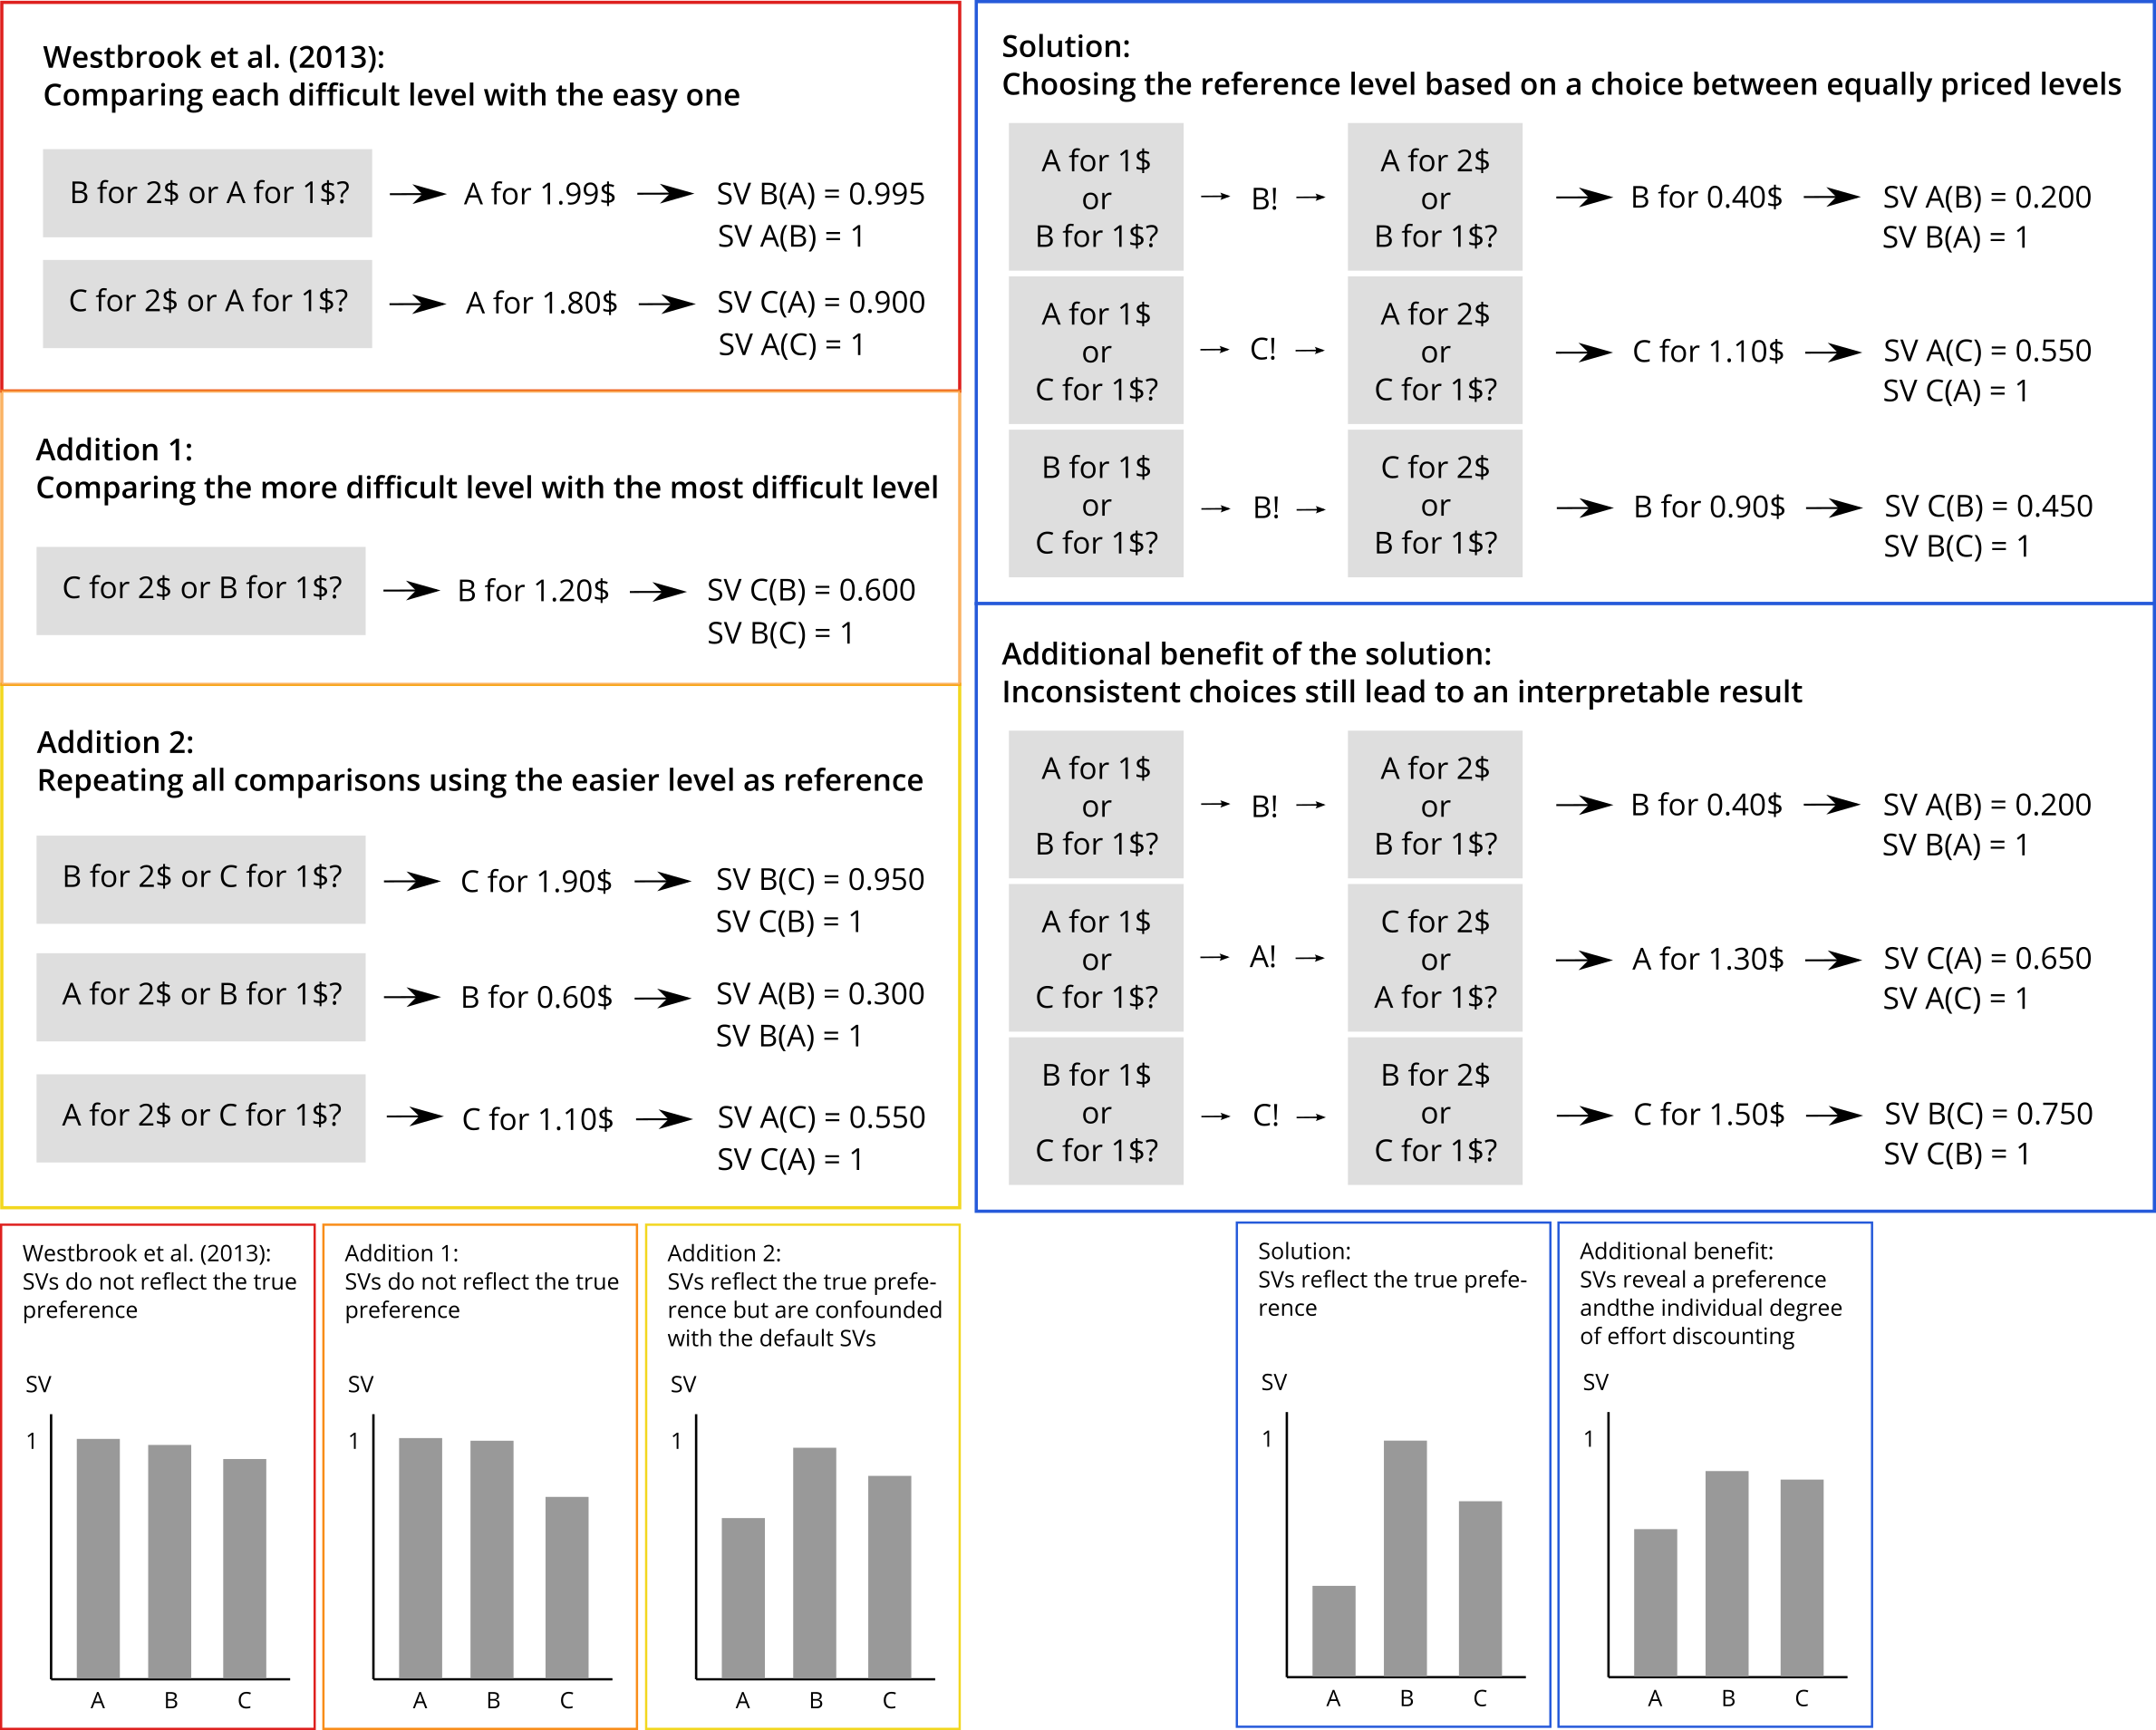
\includegraphics[width=\textwidth]{../Inkscape Figures/Paradigm_Scheme} \caption{An example for subjective values for an n-back task with three levels, returned by different modifications of the COG-ED paradigm for a hypothetical participant with the true preference 2-back > 3-back > 1-back. The grey boxes are the choice options shown to the participant. The participant's final reward value of the flexible level is displayed after the first arrow. The resulting subjective value of each level is displayed after the second arrow, in the notation "SV 3-back(1-back)" for the subjective value of 3-back when 1-back is the other choice. The Solution and Additional Benefit panel follow the same logic, but are preceded by a choice between equal rewards, and the participant's first choice indicated by an exclamation mark.}\label{fig:figure1}
\end{figure}

\hypertarget{study-procedure}{%
\subsubsection{Study procedure}\label{study-procedure}}

Healthy participants aged 18 to 30~years will be recruited using the software \emph{ORSEE}\textsuperscript{24}.
Participants will complete the personality questionnaires online and then visit the lab for two sessions one week apart.
NFC will be assessed using the 16-item short form of the Need for Cognition Scale\textsuperscript{25,26}.
Responses to each item (e.g., ``Thinking is not my idea of fun'', recoded) will be recorded on a 7-point Likert scale.
The NFC scale shows comparably high internal consistency (Cronbach's \(\alpha>.80\))\textsuperscript{26,27}.
Several other personality questionnaires will be used in this study but are the topic of the Registered Report for the second lab session\textsuperscript{17}.
A full list of measures can be found in our \href{https://github.com/ChScheffel/CAD}{Github repository}.
In the first session, participants provide informed consent and demographic data before completing the computer-based paradigm.
The paradigm starts with the \emph{n}-back levels one to four, presented sequentially with two runs per level, consisting of 64 consonants (16 targets, 48 non-targets) per run.
The levels are referred to by color (1-back black, 2-back red, 3-back blue, 4-back green) to avoid anchor effects in the effort discounting procedure.
To assess perceived task load, we will use the 6-item NASA Task Load Index (NASA-TLX)\textsuperscript{28}, where participants evaluate their subjective perception of mental load, physical load, effort, frustration, performance, and time pressure during the task on a 20-point scale.
At the end of each level, participants fill out the NASA-TLX on a tablet, plus an item with the same response scale, asking them how aversive they found this \emph{n}-back level.
After the \emph{n}-back task, participants complete the CAD paradigm on screen and are instructed to do so as realistically as possible, even though the displayed rewards will not be paid out on top of their compensation.
They are told that one of their choices will be randomly picked for the final run of \emph{n}-back, the data of which will not be analyzed as it only serves to incentivise truthful behavior and stay close to the design of Westbrook et al.\textsuperscript{7}.
After the CAD paradigm, participants will fill out a short questionnaire on the tablet, indicating whether they have adhered to the instructions (yes/no) and what the primary motivation for their decisions during the effort discounting procedure was (avoid boredom/relax/avoid effort/seek challenge/other).\\
The second session consists of an emotion regulation task with negative pictures and the instruction to suppress facial reactions, detach cognitively from the picture content, and distract oneself, respectively.
The paradigm follows the same structure of task and effort discounting procedure, but participants can decide which strategy they want to reapply in the last block.
Study data will be collected and managed using REDCap electronic data capture tools hosted at Technische Universität Dresden\textsuperscript{29,30}.

\hypertarget{sampling-plan}{%
\subsection{Sampling plan}\label{sampling-plan}}

Sample size determination was mainly based on the results of the analyses of Westbrook et al.\textsuperscript{7} (see \protect\hyperlink{DesignTableSection}{Design Table}).
The hypothesis that yielded the largest necessary sample size was a repeated measures ANOVA with within-between interaction of NFC and \emph{n}-back level influencing SVs.
Sample size analysis with \emph{G*Power}\textsuperscript{31,32} indicated that we should collect data from at least 72 participants, assuming \(\alpha=.05\) and \(\beta=.95\).
However, the sample size analysis for the hypotheses of the second lab session revealed a larger necessary sample size of 85 participants to find an effect of \(d=-0.32\) of emotion regulation on facial muscle activity with \(\alpha=.05\) and \(\beta=.95\).
To account for technical errors, noisy physiological data, or participants who indicate that they did not follow the instructions, we aim to collect about \(50\%\) more data sets than necessary, \(N=120\) in total.

\hypertarget{analysis-plan}{%
\subsection{Analysis plan}\label{analysis-plan}}

Data collection and analysis will not be performed blind to the conditions of the experiments.
We will exclude the data of a participant from all analyses, if the participant states that they did not follow the instructions, if the investigator notes that the participant misunderstood the instructions, or if the participant withdraws their consent.
No data will be replaced.
The performance measure \emph{d'} will be computed as the difference of the \emph{z}-transformed hit rate and the \emph{z}-transformed false alarm rate\textsuperscript{33}.
Reaction time (RT) data will be trimmed by excluding all trials with responses faster than 100~ms, as the relevant cognitive processes cannot have been completed before\textsuperscript{34,35}.
Aggregated RT values will be described using the median and the median of absolute deviation (\(MAD\)) as robust estimates of center and variability, respectively\textsuperscript{36}.
Error- and post-error trials will be excluded, because RT in the latter is longer due to more cautious behavior\textsuperscript{37,38}.
To test our hypotheses, we will perform a series of rmANOVAs and an MLM with orthogonal sum-to-zero contrasts in order to meaningfully interpret results\textsuperscript{39}.

\emph{Manipulation check.}
Declining performance will be investigated by calculating an rmANOVA with six paired contrasts comparing \emph{d'} between two levels of 1- to 4-back at a time.
Another rmANOVA with six paired contrasts will be computed to compare the median RT between two levels of 1- to 4-back at a time.
To investigate changes in NASA-TLX ratings, six rmANOVAs will be computed, one for each NASA-TLX subscale, and each with six paired contrasts comparing the ratings between two levels of 1- to 4-back at a time.

\emph{Subjective values.}
For each effort discounting round, the SV of the fixed level will be calculated by adding or subtracting the last adjustment of 0.02~€ from the last monetary value of the flexible level, depending on the participant's last choice, and dividing this value by 2~€.
This yields an SV between 0 and 1 for the fixed compared with the flexible level, while the SV of the flexible level is 1.
The closer the SV of the fixed level is to 0, the stronger the preference for the flexible level.
All SVs of each level will be averaged to compute one ``global'' SV for each level.
An rmANOVA with four different contrasts will be computed to investigate the association of SVs and the \emph{n}-back levels: Declining linear (3,1,-1,-3), ascending quadratic (-1,1,1,-1), declining logistic (3,2,-2,-3), and positively skewed normal (1,2,-1,-2).
Depending on whether the linear or one of the other three contrasts fits the curve best, we will apply a linear or nonlinear multi-level model in the next step, respectively.

To determine the influence of task performance on the association of SVs and \emph{n}-back level, we will perform MLM.
We will apply restricted maximum likelihood (REML) to fit the model.
As an effect size measure for random effects we will firstly calculate the intraclass correlation (ICC), which displays the proportion of variance that is explained by differences between persons.
Second, we will estimate a random slopes model of n-back level (level 1, fixed and random factor: 0-back, 1-back, 2-back, 3-back) predicting SV nested within subjects.
As Mussel et al.\textsuperscript{40} could show, participants with high versus low NFC not only have a more shallow decline in performance with higher n-back levels, but show a demand-specific increase in EEG theta oscillations, which has been associated with mental effort.
We control for performance, i.e., \emph{d'} (level 1, fixed factor, continuous), median RT (level 1, fixed factor, continuous) in order to eliminate a possible influence of declining performance on SV ratings.
\[
SV \sim level\ + d' + median RT + (level|subject)
\]
Level-1-predictors will be centered within cluster as recommended by Enders \& Tofighi\textsuperscript{41}.
By this, the model yields interpretable parameter estimates.
If necessary, we will adjusted the optimization algorithm to improve model fit.
We will visually inspect the residuals of the model for evidence to perform model criticism.
This will be done by excluding all data points with absolute standardized residuals above 3 SD.
As effect size measures, we will calculate pseudo \emph{R²} for our model and \emph{f²} to estimate the effect of n-back level according to Lorah\textsuperscript{42}.

The association of SVs and NFC will be examined with an rmANOVA.
We will subtract the SV of 1- from 2-back, 2- from 3-back, and 3- from 4-back per participant, yielding three SV difference scores per participant.
The sample will be divided into participants with low and high NFC using a median split.
We will then compute an rmANOVA with the within-factor n-back level and the between-factor NFC group to determine whether there is a main effect of level and/or group, and/or an interaction between level and group on the SV difference scores.
Post-hoc tests will be computed depending on which effect reaches significance at \(p<.01\).
To ensure the validity of this association, we will conduct a specification curve analysis\textsuperscript{43}, which will include 63 possible preprocessing pipelines of the RT data.
These pipelines specify which transformation was applied (none, log, inverse, or square-root), which outliers were excluded (none, 2, 2.5, or 3~\(MAD\) from the median, RTs below 100~or~200~ms), and across which dimensions the transformations and exclusions were applied (across/within subjects and across/within \emph{n}-back levels).
The rmANOVA will be run with each of the 63~pipelines, which will also include our main pipeline (untransformed data, exclusion of RTs below 100~ms).
The ratio of pipelines that lead to significant versus non-significant effects will provide an indication of how robust the effect actually is.

The association of subjective task load with NFC will be examined similarly.
We will calculate NASA-TLX sum scores per participant per level and compute an rmANOVA with the within-factor n-back level and the between-factor NFC group, and apply post-hoc tests based on which effect reaches significance at \(p<.01\).
And the association of subjective aversiveness of the task with NFC will be examined with difference scores as well, since we expect this curve to mirror the SV curve, i.e.~as the SV rises, the aversiveness declines, and vice versa.
We will subtract the aversiveness ratings of 1- from 2-back, 2- from 3-back, and 3- from 4-back per participant, yielding three aversiveness difference scores per participant.
Then, we will compute an rmANOVA with the within-factor n-back level and the between-factor NFC group, and apply post-hoc tests based on which effect reaches significance at \(p<.01\).

The results of each analysis will be assessed on the basis of both \(p\)-value and the Bayes factor \(BF10\), calculated with the \emph{BayesFactor} package\textsuperscript{23} using the default prior widths of the functions \emph{anovaBF}, \emph{lmBF} and \emph{ttestBF}.
We will consider a \(BF10\) close to or above 3/10 as moderate/strong evidence for the alternative hypothesis, and a \(BF10\) close to or below .33/.10 as moderate/strong evidence for the null hypothesis\textsuperscript{44}.

\hypertarget{pilot-data}{%
\subsection{Pilot data}\label{pilot-data}}

The sample of the pilot study consisted of \(N=15\) participants (53.30\% female, \(M=24.43\) (\(SD=3.59\))~years old).
One participant's data was removed because they misunderstood the instruction.
Due to a technical error the subjective task load data of one participant was incomplete, so the hypotheses involving the NASA Task Load Index were analyzed with \(n=14\) data sets.
The results showed increases in subjective and objective task load measures with higher \emph{n}-back level.
Importantly, SVs were lower for higher \emph{n}-back levels, but not different between 1- and 2-back, which shows that the easiest level is not universally preferred.
The LMM revealed \emph{n}-back level as a reliable predictor of SV, even after controlling for declining task performance (\emph{d'} and median RT).
NASA-TLX scores were higher with higher \emph{n}, and lower for the group with lower NFC scores, but NFC and \emph{n}-back level did not interact.
All results are detailed in the Supplementary Material.

\hypertarget{data-availability}{%
\subsection{Data availability}\label{data-availability}}

The data of this study can be downloaded from \href{https://osf.io/vnj8x/}{osf.io/vnj8x/}.

\hypertarget{code-availability}{%
\subsection{Code availability}\label{code-availability}}

The paradigm code as well as the R Markdown file used to analyze the data and write this document is available at \href{https://github.com/ChScheffel/CAD}{github.com/ChScheffel/CAD}.

\newpage

\hypertarget{references}{%
\section{References}\label{references}}

\begingroup
\setlength{\parindent}{-0.5in}
\setlength{\leftskip}{0.5in}

\hypertarget{refs}{}
\begin{CSLReferences}{0}{0}
\leavevmode\vadjust pre{\hypertarget{ref-Botvinick2009}{}}%
\CSLLeftMargin{1. }%
\CSLRightInline{Botvinick, M. M., Huffstetler, S. \& McGuire, J. T. \href{https://doi.org/10.3758/CABN.9.1.16}{Effort discounting in human nucleus accumbens}. \emph{Cognitive, affective \& behavioral neuroscience} \textbf{9}, 16--27 (2009).}

\leavevmode\vadjust pre{\hypertarget{ref-Kool2018}{}}%
\CSLLeftMargin{2. }%
\CSLRightInline{Kool, W. \& Botvinick, M. \href{https://doi.org/10.1038/s41562-018-0401-9}{Mental labour}. \emph{Nature Human Behaviour} \textbf{2}, 899--908 (2018).}

\leavevmode\vadjust pre{\hypertarget{ref-Mackworth1959}{}}%
\CSLLeftMargin{3. }%
\CSLRightInline{Mackworth, J. F. \href{https://doi.org/10.1037/h0049090}{Paced memorizing in a continuous task}. \emph{Journal of Experimental Psychology} \textbf{58}, 206--211 (1959).}

\leavevmode\vadjust pre{\hypertarget{ref-Jaeggi2010}{}}%
\CSLLeftMargin{4. }%
\CSLRightInline{Jaeggi, S. M., Buschkuehl, M., Perrig, W. J. \& Meier, B. \href{https://doi.org/10.1080/09658211003702171}{The concurrent validity of the {N}-back task as a working memory measure}. \emph{Memory} \textbf{18}, 394--412 (2010).}

\leavevmode\vadjust pre{\hypertarget{ref-Jonides1997}{}}%
\CSLLeftMargin{5. }%
\CSLRightInline{Jonides, J. \emph{et al.} \href{https://doi.org/10.1162/jocn.1997.9.4.462}{Verbal {Working} {Memory} {Load} {Affects} {Regional} {Brain} {Activation} as {Measured} by {PET}}. \emph{Journal of Cognitive Neuroscience} \textbf{9}, 462--475 (1997).}

\leavevmode\vadjust pre{\hypertarget{ref-Owen2005}{}}%
\CSLLeftMargin{6. }%
\CSLRightInline{Owen, A. M., McMillan, K. M., Laird, A. R. \& Bullmore, E. \href{https://doi.org/10.1002/hbm.20131}{N-back working memory paradigm: A meta-analysis of normative functional neuroimaging studies}. \emph{Human Brain Mapping} \textbf{25}, 46--59 (2005).}

\leavevmode\vadjust pre{\hypertarget{ref-Westbrook2013}{}}%
\CSLLeftMargin{7. }%
\CSLRightInline{Westbrook, A., Kester, D. \& Braver, T. S. \href{https://doi.org/10.1371/journal.pone.0068210}{What is the subjective cost of cognitive effort? {Load}, trait, and aging effects revealed by economic preference}. \emph{PLOS ONE} \textbf{8}, e68210 (2013).}

\leavevmode\vadjust pre{\hypertarget{ref-Cacioppo1982}{}}%
\CSLLeftMargin{8. }%
\CSLRightInline{Cacioppo, J. T. \& Petty, R. E. \href{https://doi.org/10.1037//0022-3514.42.1.116}{The {Need} for {Cognition}}. \emph{Journal of Personality and Social Psychology} \textbf{42}, 116--131 (1982).}

\leavevmode\vadjust pre{\hypertarget{ref-Wu2021}{}}%
\CSLLeftMargin{9. }%
\CSLRightInline{Wu, R., Ferguson, A. \& Inzlicht, M. \emph{Do humans prefer cognitive effort over doing nothing?} \url{https://psyarxiv.com/d2gkf/} (2021) doi:\href{https://doi.org/10.31234/osf.io/d2gkf}{10.31234/osf.io/d2gkf}.}

\leavevmode\vadjust pre{\hypertarget{ref-Bertrams2012}{}}%
\CSLLeftMargin{10. }%
\CSLRightInline{Bertrams, A. \& Dickhäuser, O. \href{https://doi.org/10.1027/1614-0001/a000081}{Passionate thinkers feel better}. \emph{Journal of Individual Differences} \textbf{33}, 69--75 (2012).}

\leavevmode\vadjust pre{\hypertarget{ref-Nishiguchi2016}{}}%
\CSLLeftMargin{11. }%
\CSLRightInline{Nishiguchi, Y., Takano, K. \& Tanno, Y. \href{https://doi.org/10.1016/j.psychres.2016.04.092}{The {Need} for {Cognition} mediates and moderates the association between depressive symptoms and impaired {Effortful} {Control}}. \emph{Psychiatry Research} \textbf{241}, 8--13 (2016).}

\leavevmode\vadjust pre{\hypertarget{ref-Xu2021}{}}%
\CSLLeftMargin{12. }%
\CSLRightInline{Xu, P. \& Cheng, J. \href{https://doi.org/10.1016/j.paid.2021.110706}{Individual differences in social distancing and mask-wearing in the pandemic of {COVID}-19: {The} role of need for cognition, self-control and risk attitude}. \emph{Personality and Individual Differences} \textbf{175}, 110706 (2021).}

\leavevmode\vadjust pre{\hypertarget{ref-Kramer2021}{}}%
\CSLLeftMargin{13. }%
\CSLRightInline{Kramer, A.-W., Van Duijvenvoorde, A. C. K., Krabbendam, L. \& Huizenga, H. M. \href{https://doi.org/10.1016/j.cogdev.2020.100978}{Individual differences in adolescents' willingness to invest cognitive effort: {Relation} to need for cognition, motivation and cognitive capacity}. \emph{Cognitive Development} \textbf{57}, 100978 (2021).}

\leavevmode\vadjust pre{\hypertarget{ref-Crawford2021}{}}%
\CSLLeftMargin{14. }%
\CSLRightInline{Crawford, J. L., Eisenstein, S. A., Peelle, J. E. \& Braver, T. S. \href{https://doi.org/10.1186/s41235-021-00272-7}{Domain-general cognitive motivation: Evidence from economic decision-making}. \emph{Cognitive Research: Principles and Implications} \textbf{6}, 4 (2021).}

\leavevmode\vadjust pre{\hypertarget{ref-Culbreth2016}{}}%
\CSLLeftMargin{15. }%
\CSLRightInline{Culbreth, A., Westbrook, A. \& Barch, D. \href{https://doi.org/10.1037/abn0000153}{Negative symptoms are associated with an increased subjective cost of cognitive effort}. \emph{Journal of Abnormal Psychology} \textbf{125}, 528--536 (2016).}

\leavevmode\vadjust pre{\hypertarget{ref-Westbrook2019}{}}%
\CSLLeftMargin{16. }%
\CSLRightInline{Westbrook, A., Lamichhane, B. \& Braver, T. \href{https://doi.org/10.1523/jneurosci.3071-18.2019}{The subjective value of cognitive effort is encoded by a domain-general valuation network}. \emph{The Journal of Neuroscience} \textbf{39}, 3934--3947 (2019).}

\leavevmode\vadjust pre{\hypertarget{ref-ScheffelZerna2022}{}}%
\CSLLeftMargin{17. }%
\CSLRightInline{Scheffel, C., Zerna, J., Gärtner, A., Dörfel, D. \& Strobel, A. \href{https://psyarxiv.com/wr8qx}{Estimating individual subjective values of emotion regulation strategies}. (2022).}

\leavevmode\vadjust pre{\hypertarget{ref-Simmons2012}{}}%
\CSLLeftMargin{18. }%
\CSLRightInline{Simmons, J. P., Nelson, L. D. \& Simonsohn, U. A 21 word solution. (2012) doi:\href{https://doi.org/10.2139/ssrn.2160588}{10.2139/ssrn.2160588}.}

\leavevmode\vadjust pre{\hypertarget{ref-Peirce2019}{}}%
\CSLLeftMargin{19. }%
\CSLRightInline{Peirce, J. \emph{et al.} \href{https://doi.org/10.3758/s13428-018-01193-y}{{PsychoPy2}: {Experiments} in behavior made easy}. \emph{Behavior Research Methods} \textbf{51}, 195--203 (2019).}

\leavevmode\vadjust pre{\hypertarget{ref-RCT2020}{}}%
\CSLLeftMargin{20. }%
\CSLRightInline{R Core Team. \emph{\href{https://www.R-project.org/}{R: {A} language and environment for statistical computing}}. (R Foundation for Statistical Computing, 2020).}

\leavevmode\vadjust pre{\hypertarget{ref-RStudioTeam2020}{}}%
\CSLLeftMargin{21. }%
\CSLRightInline{RStudio Team. \href{http://www.rstudio.com}{{RStudio}: {Integrated} development for {R}}. (2020).}

\leavevmode\vadjust pre{\hypertarget{ref-Singmann2021}{}}%
\CSLLeftMargin{22. }%
\CSLRightInline{Singmann, H., Bolker, B., Westfall, J., Aust, F. \& Ben-Shachar, M. S. \emph{\href{https://CRAN.R-project.org/package=afex}{Afex: {A}nalysis of factorial experiments}}. (2021).}

\leavevmode\vadjust pre{\hypertarget{ref-Morey2021}{}}%
\CSLLeftMargin{23. }%
\CSLRightInline{Morey, R. D. \& Rouder, J. N. \emph{\href{https://CRAN.R-project.org/package=BayesFactor}{{BayesFactor}: {Computation} of {Bayes} factors for common designs}}. (2021).}

\leavevmode\vadjust pre{\hypertarget{ref-Greiner2015}{}}%
\CSLLeftMargin{24. }%
\CSLRightInline{Greiner, B. \href{https://doi.org/10.1007/s40881-015-0004-4}{Subject pool recruitment procedures: {Organizing} experiments with {ORSEE}}. \emph{Journal of the Economic Science Association} \textbf{1}, 114--125 (2015).}

\leavevmode\vadjust pre{\hypertarget{ref-Cacioppo1984}{}}%
\CSLLeftMargin{25. }%
\CSLRightInline{Cacioppo, J. T., Petty, R. E. \& Kao, C. F. \href{https://doi.org/10.1207/s15327752jpa4803_13}{The {Efficient} {Assessment} of {Need} for {Cognition}}. \emph{Journal of Personality Assessment} \textbf{48}, 306--307 (1984).}

\leavevmode\vadjust pre{\hypertarget{ref-Bless1994}{}}%
\CSLLeftMargin{26. }%
\CSLRightInline{Bless, H., Wänke, M., Bohner, G., Fellhauer, R. F. \& Schwarz, N. \href{https://doi.org/1779110}{Need for {Cognition}: {Eine} {Skala} zur {Erfassung} von {Engagement} und {Freude} bei {Denkaufgaben}}. \emph{Zeitschrift für Sozialpsychologie} \textbf{25}, (1994).}

\leavevmode\vadjust pre{\hypertarget{ref-Fleischhauer2010}{}}%
\CSLLeftMargin{27. }%
\CSLRightInline{Fleischhauer, M. \emph{et al.} \href{https://doi.org/10.1177/0146167209351886}{Same or different? {Clarifying} the relationship of need for cognition to personality and intelligence}. \emph{Personality \& Social Psychology Bulletin} \textbf{36}, 82--96 (2010).}

\leavevmode\vadjust pre{\hypertarget{ref-Hart1988}{}}%
\CSLLeftMargin{28. }%
\CSLRightInline{Hart, S. G. \& Staveland, L. E. \href{https://doi.org/10.1016/S0166-4115(08)62386-9}{Development of {NASA}-{TLX} ({Task} {Load} {Index}): {Results} of empirical and theoretical research}. \textbf{52}, 139--183 (1988).}

\leavevmode\vadjust pre{\hypertarget{ref-Harris2009}{}}%
\CSLLeftMargin{29. }%
\CSLRightInline{Harris, P. A. \emph{et al.} \href{https://doi.org/10.1016/j.jbi.2008.08.010}{Research electronic data capture ({REDCap})---{A} metadata-driven methodology and workflow process for providing translational research informatics support}. \emph{Journal of Biomedical Informatics} \textbf{42}, 377--381 (2009).}

\leavevmode\vadjust pre{\hypertarget{ref-Harris2019}{}}%
\CSLLeftMargin{30. }%
\CSLRightInline{Harris, P. A. \emph{et al.} \href{https://doi.org/10.1016/j.jbi.2019.103208}{The {REDCap} consortium: {Building} an international community of software platform partners}. \emph{Journal of Biomedical Informatics} \textbf{95}, 103208 (2019).}

\leavevmode\vadjust pre{\hypertarget{ref-Faul2007}{}}%
\CSLLeftMargin{31. }%
\CSLRightInline{Faul, F., Erdfelder, E., Lang, A.-G. \& Buchner, A. \href{https://doi.org/10.3758/BF03193146}{G*{Power} 3: {A} flexible statistical power analysis program for the social, behavioral, and biomedical sciences}. \emph{Behavior Research Methods} \textbf{39}, 175--191 (2007).}

\leavevmode\vadjust pre{\hypertarget{ref-Faul2009}{}}%
\CSLLeftMargin{32. }%
\CSLRightInline{Faul, F., Erdfelder, E., Buchner, A. \& Lang, A.-G. \href{https://doi.org/10.3758/BRM.41.4.1149}{Statistical power analyses using {G}*{Power} 3.1: {Tests} for correlation and regression analyses}. \emph{Behavior Research Methods} \textbf{41}, 1149--1160 (2009).}

\leavevmode\vadjust pre{\hypertarget{ref-Macmillan1990}{}}%
\CSLLeftMargin{33. }%
\CSLRightInline{Macmillan, N. A. \& Creelman, C. D. \href{https://doi.org/10.1037/0033-2909.107.3.401}{Response bias: {Characteristics} of detection theory, threshold theory, and "nonparametric" indexes}. \emph{Psychological Bulletin} \textbf{107}, 401--413 (1990).}

\leavevmode\vadjust pre{\hypertarget{ref-Whelan2008}{}}%
\CSLLeftMargin{34. }%
\CSLRightInline{Whelan, R. \href{https://doi.org/10.1007/BF03395630}{Effective {Analysis} of {Reaction} {Time} {Data}}. \emph{The Psychological Record} \textbf{58}, 475--482 (2008).}

\leavevmode\vadjust pre{\hypertarget{ref-Berger2021}{}}%
\CSLLeftMargin{35. }%
\CSLRightInline{Berger, A. \& Kiefer, M. \href{https://doi.org/10.3389/fpsyg.2021.675558}{Comparison of {Different} {Response} {Time} {Outlier} {Exclusion} {Methods}: {A} {Simulation} {Study}}. \emph{Frontiers in Psychology} \textbf{12}, 2194 (2021).}

\leavevmode\vadjust pre{\hypertarget{ref-Lachaud2011}{}}%
\CSLLeftMargin{36. }%
\CSLRightInline{Lachaud, C. M. \& Renaud, O. \href{https://doi.org/10.1017/s0142716410000457}{A tutorial for analyzing human reaction times: {How} to filter data, manage missing values, and choose a statistical model}. \emph{Applied Psycholinguistics} \textbf{32}, 389--416 (2011).}

\leavevmode\vadjust pre{\hypertarget{ref-Dutilh2012}{}}%
\CSLLeftMargin{37. }%
\CSLRightInline{Dutilh, G. \emph{et al.} \href{https://doi.org/10.3758/s13414-011-0243-2}{Testing theories of post-error slowing}. \emph{Attention, Perception, \& Psychophysics} \textbf{74}, 454--465 (2012).}

\leavevmode\vadjust pre{\hypertarget{ref-Houtman2012}{}}%
\CSLLeftMargin{38. }%
\CSLRightInline{Houtman, F., Castellar, E. N. \& Notebaert, W. \href{https://doi.org/10.1080/20445911.2011.617301}{Orienting to errors with and without immediate feedback}. \emph{Journal of Cognitive Psychology} \textbf{24}, 278--285 (2012).}

\leavevmode\vadjust pre{\hypertarget{ref-Singmann2019}{}}%
\CSLLeftMargin{39. }%
\CSLRightInline{Singmann, H. \& Kellen, D. An introduction to mixed models for experimental psychology. in \emph{New methods in cognitive psychology} 4--31 (Routledge, 2019). doi:\href{https://doi.org/10.4324/9780429318405-2}{10.4324/9780429318405-2}.}

\leavevmode\vadjust pre{\hypertarget{ref-Mussel2016}{}}%
\CSLLeftMargin{40. }%
\CSLRightInline{Mussel, P., Ulrich, N., Allen, J. J. B., Osinsky, R. \& Hewig, J. \href{https://doi.org/10.1038/srep29245}{Patterns of theta oscillation reflect the neural basis of individual differences in epistemic motivation}. \emph{Scientific Reports} \textbf{6}, (2016).}

\leavevmode\vadjust pre{\hypertarget{ref-Enders2007}{}}%
\CSLLeftMargin{41. }%
\CSLRightInline{Enders, C. K. \& Tofighi, D. \href{https://doi.org/10.1037/1082-989x.12.2.121}{Centering predictor variables in cross-sectional multilevel models: {A} new look at an old issue.} \emph{Psychological Methods} \textbf{12}, 121--138 (2007).}

\leavevmode\vadjust pre{\hypertarget{ref-Lorah2018}{}}%
\CSLLeftMargin{42. }%
\CSLRightInline{Lorah, J. \href{https://doi.org/10.1186/s40536-018-0061-2}{Effect size measures for multilevel models: Definition, interpretation, and {TIMSS} example}. \emph{Large-scale Assessments in Education} \textbf{6}, (2018).}

\leavevmode\vadjust pre{\hypertarget{ref-Simonsohn2020}{}}%
\CSLLeftMargin{43. }%
\CSLRightInline{Simonsohn, U., Simmons, J. P. \& Nelson, L. D. \href{https://doi.org/10.1038/s41562-020-0912-z}{Specification curve analysis}. \emph{Nature Human Behaviour} \textbf{4}, 1208--1214 (2020).}

\leavevmode\vadjust pre{\hypertarget{ref-Wetzels2015}{}}%
\CSLLeftMargin{44. }%
\CSLRightInline{Wetzels, R., Ravenzwaaij, D. van \& Wagenmakers, E.-J. Bayesian analysis. 1--11 (2015) doi:\href{https://doi.org/10.1002/9781118625392.wbecp453}{10.1002/9781118625392.wbecp453}.}

\end{CSLReferences}

\endgroup

\newpage

\hypertarget{acknowledgements}{%
\section{Acknowledgements}\label{acknowledgements}}

This research is partly funded by the German Research Foundation (DFG) as part of the Collaborative Research Center (CRC) 940, and partly funded by centralized funds of the Faculty of Psychology at Technische Universität Dresden.
The funders have/had no role in study design, data collection and analysis, decision to publish or preparation of the manuscript.

\hypertarget{author-contributions}{%
\section{Author Contributions}\label{author-contributions}}

JZ, CS, and AS conceptualized the study and acquired funding.
JZ and CS developed the methodology, investigated, administered the project, and wrote the software.
JZ and CK did the formal analysis, visualized the results, and prepared the original draft.
All authors reviewed, edited, and approved the final version of the manuscript.

\hypertarget{competing-interests}{%
\section{Competing Interests}\label{competing-interests}}

The authors declare no competing interests.

\newpage
\setcounter{figure}{0}

\hypertarget{figures-and-figure-captions}{%
\section{Figures and figure Captions}\label{figures-and-figure-captions}}

\begin{figure}
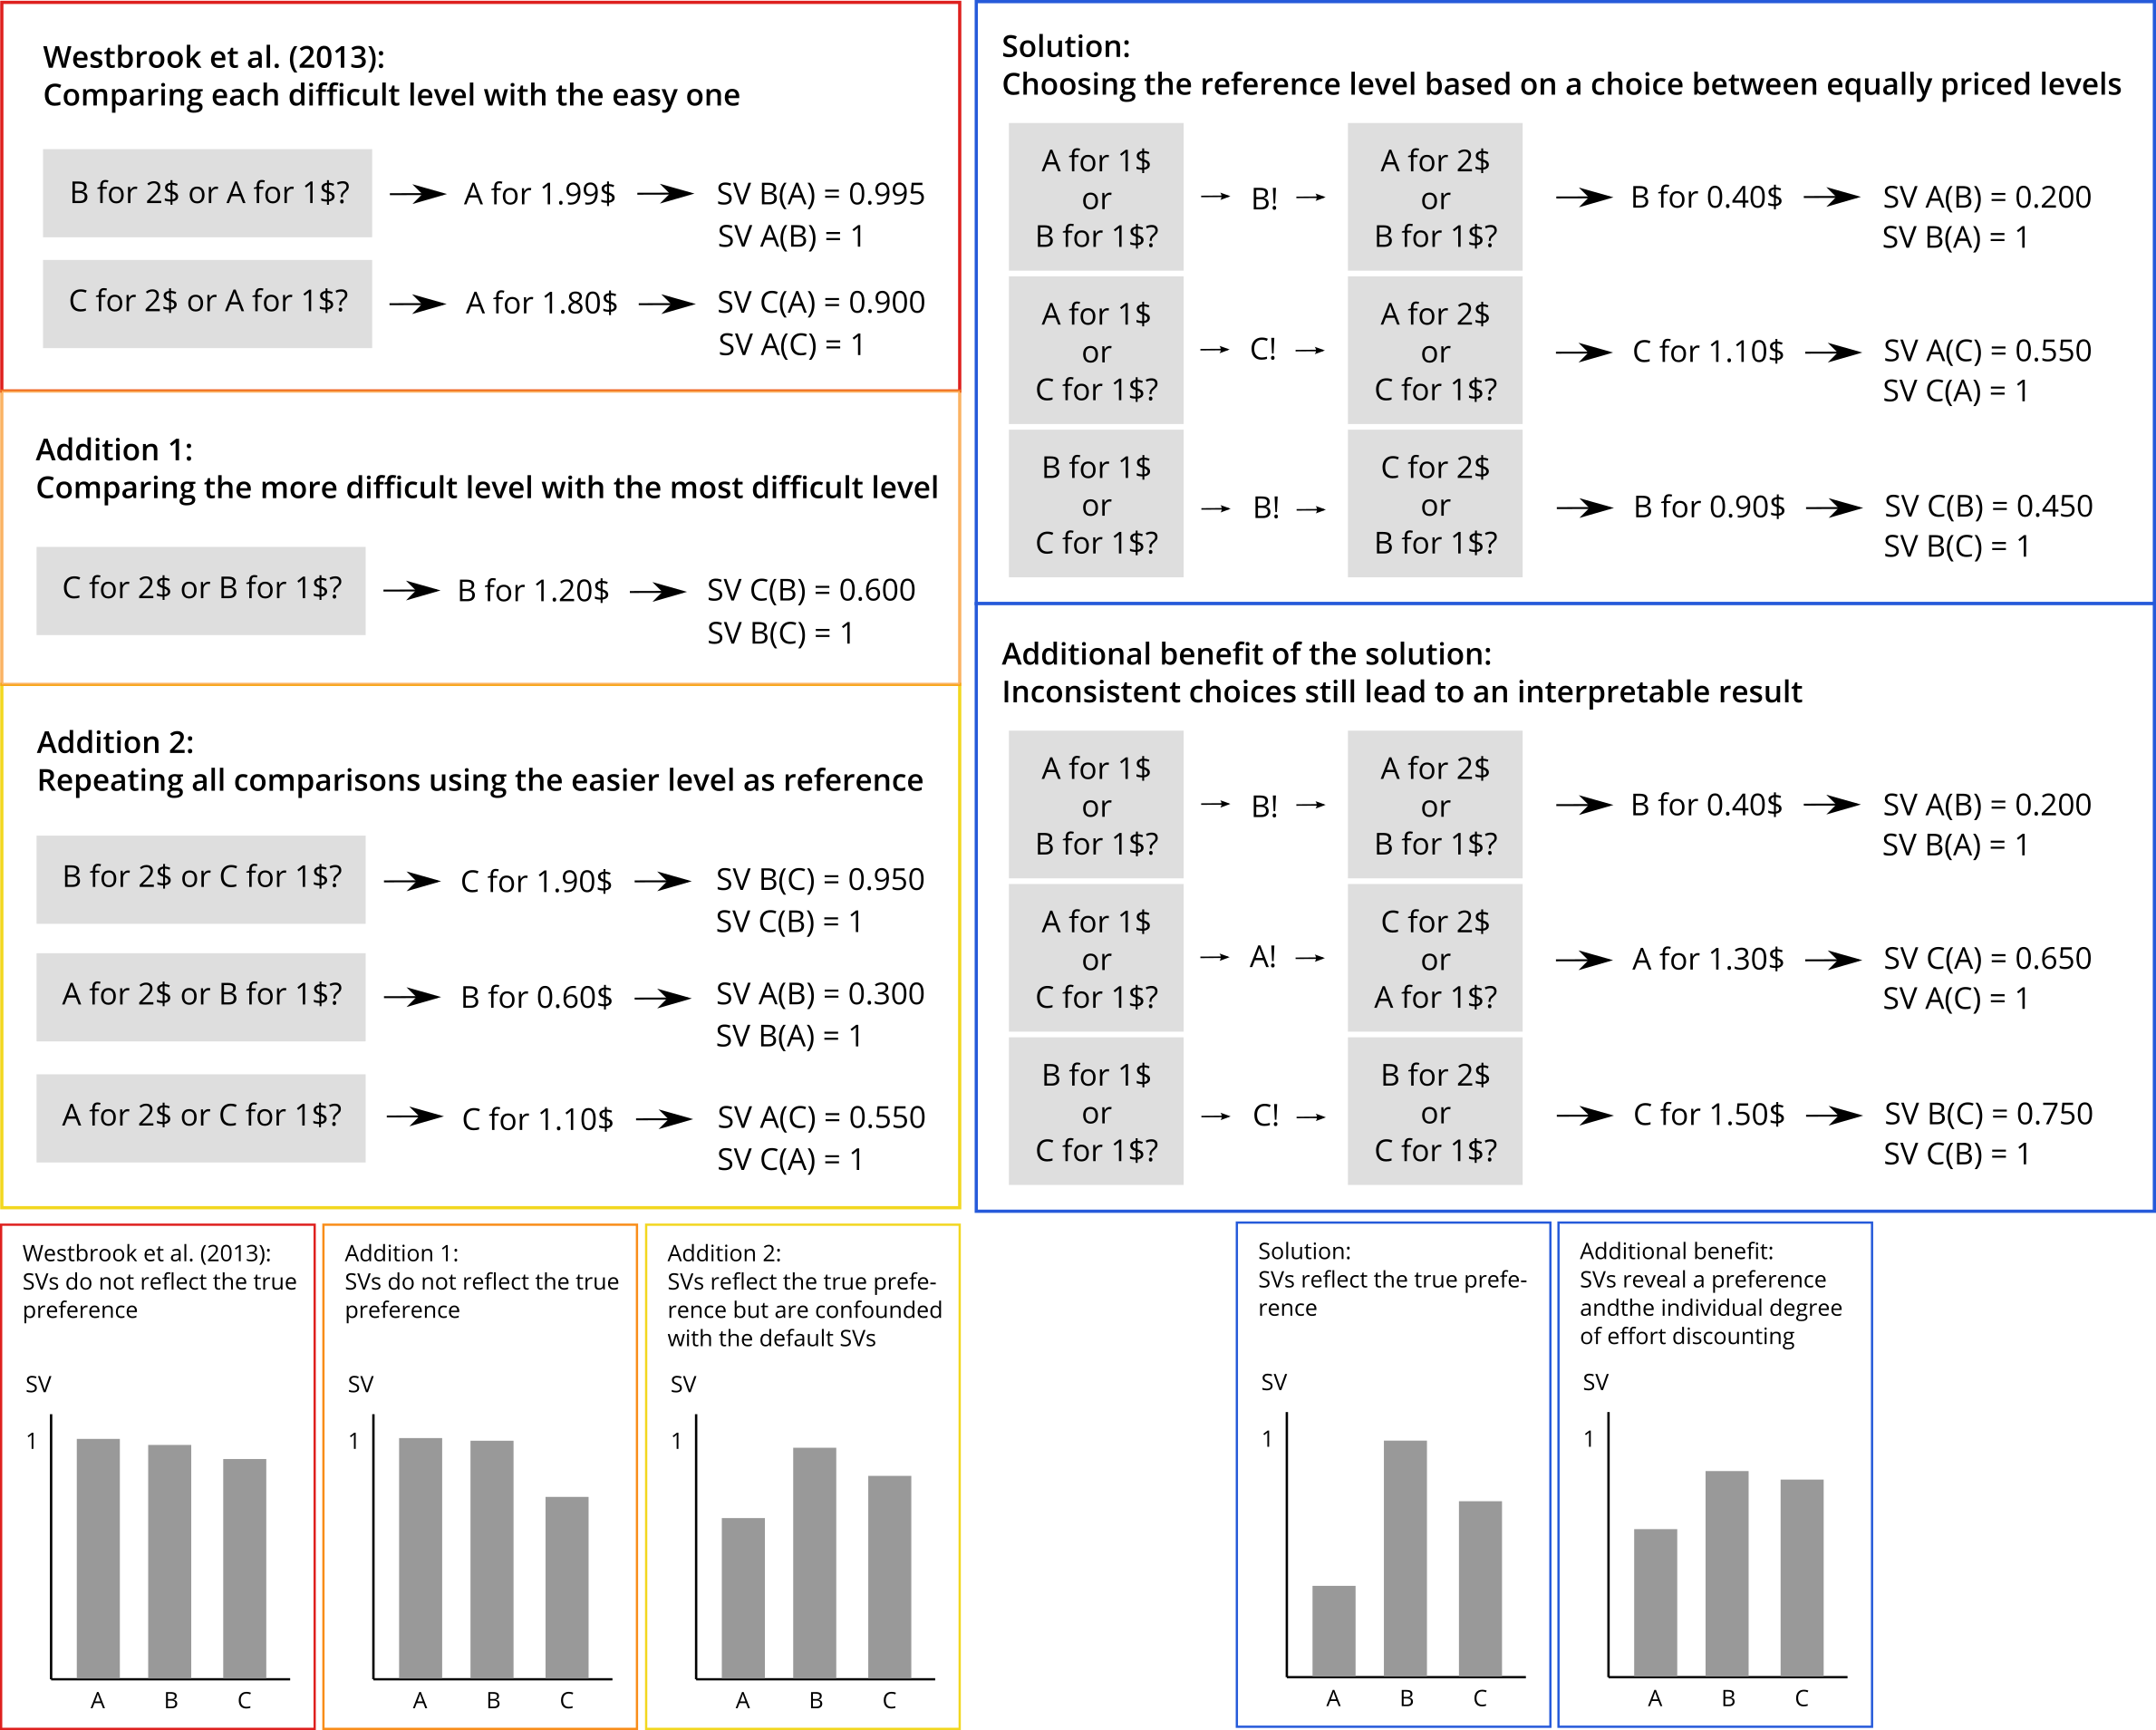
\includegraphics[width=\textwidth]{../Inkscape Figures/Paradigm_Scheme} \caption{ }\label{fig:figure1appendix}
\end{figure}

\emph{Figure 1.} An example for subjective values for an n-back task with three levels, returned by different modifications of the COG-ED paradigm for a hypothetical participant with the true preference 2-back \textgreater{} 3-back \textgreater{} 1-back. The grey boxes are the choice options shown to the participant. The participant's final reward value of the flexible level is displayed after the first arrow. The resulting subjective value of each level is displayed after the second arrow, in the notation ``SV 3-back(1-back)'' for the subjective value of 3-back when 1-back is the other choice. The Solution and Additional Benefit panel follow the same logic, but are preceded by a choice between equal rewards, and the participant's first choice indicated by an exclamation mark.

\newpage

\hypertarget{DesignTableSection}{%
\section{Design Table}\label{DesignTableSection}}

(Starts on next page)

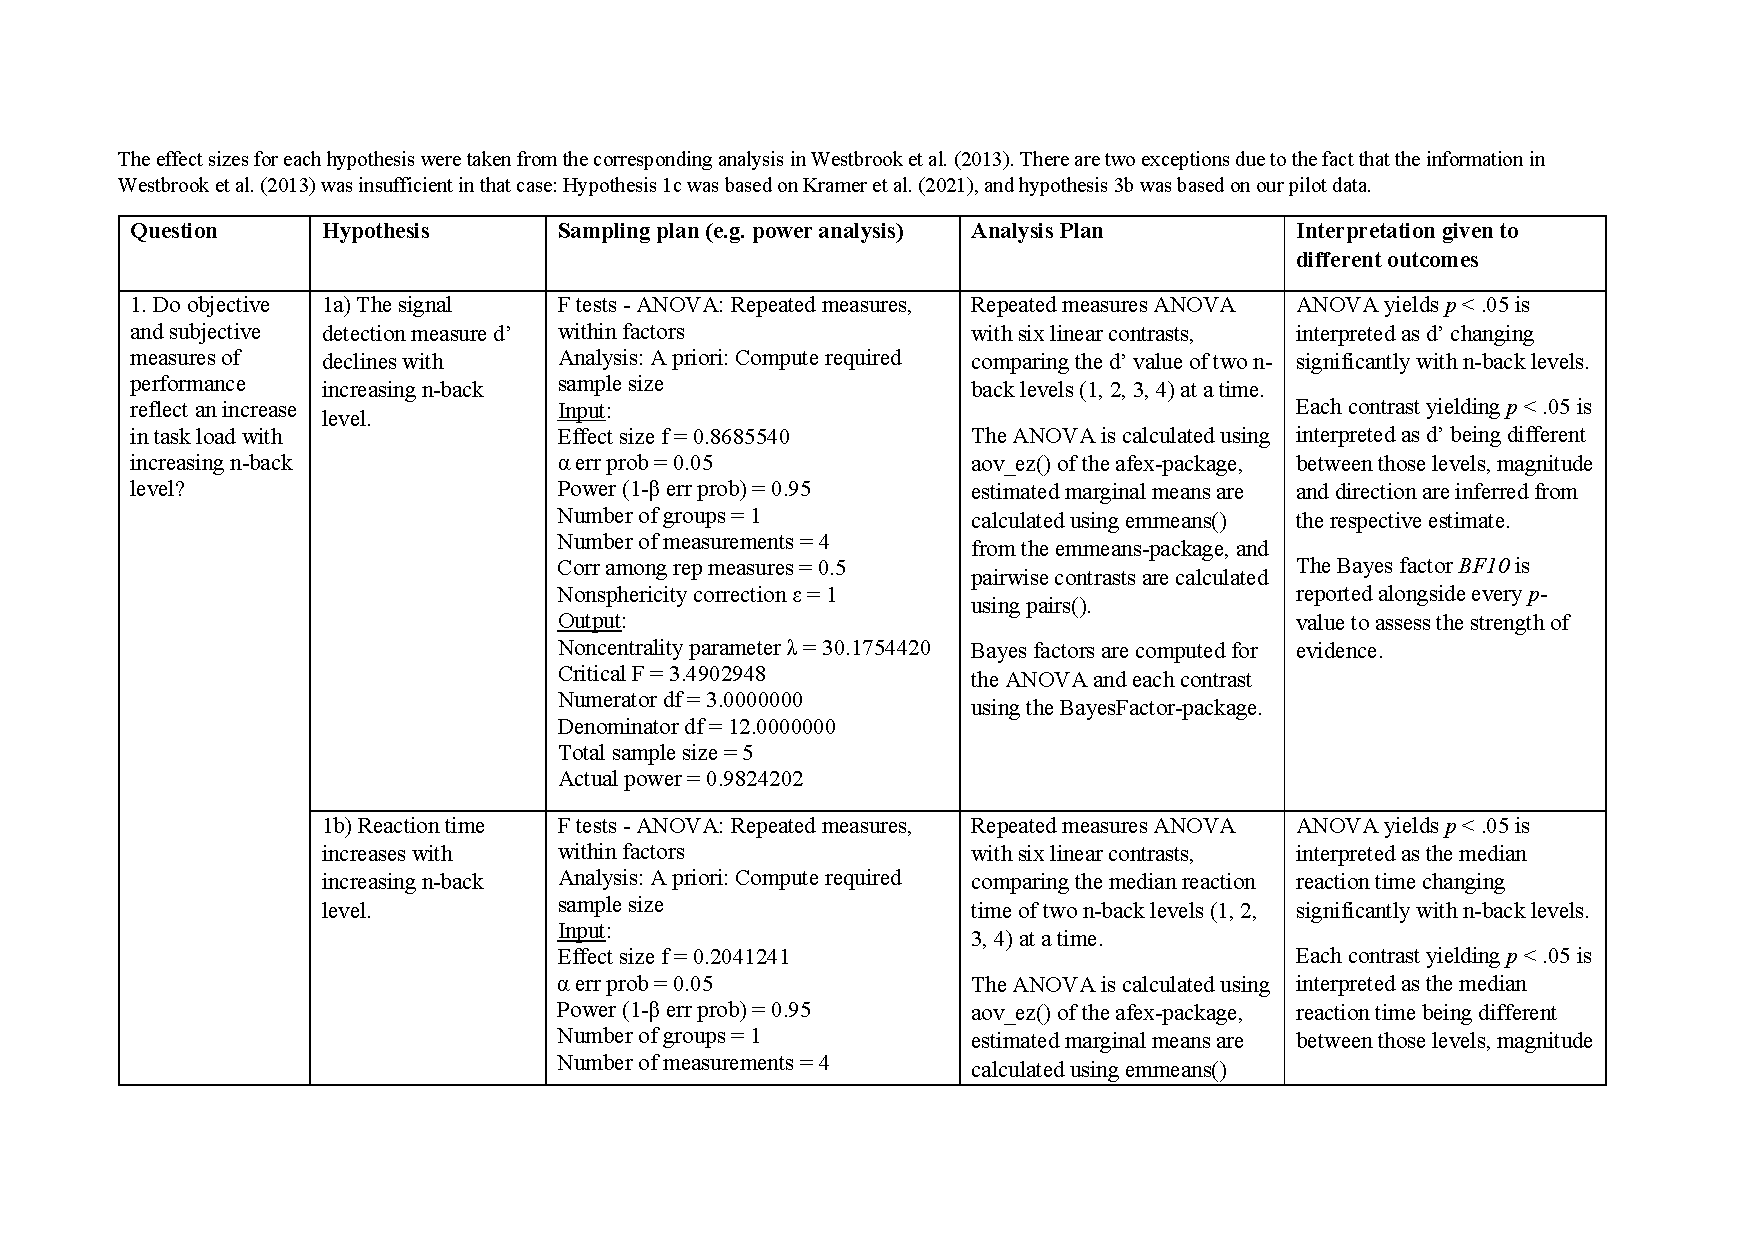
\includepdf[pages={-},landscape=true]{Design_Table_T1.pdf}

\newpage

\hypertarget{supplement}{%
\section{Supplement}\label{supplement}}

\counterwithin{figure}{section}
\counterwithin{table}{section}
\setcounter{section}{19}
\setcounter{figure}{0}
\setcounter{table}{0}

\hypertarget{results-of-the-pilot-study}{%
\subsection{Results of the pilot study}\label{results-of-the-pilot-study}}

\hypertarget{hypothesis-1a-the-signal-detection-measure-d-declines-with-increasing-n-back-level.}{%
\subsection{Hypothesis 1a: The signal detection measure d' declines with increasing n-back level.}\label{hypothesis-1a-the-signal-detection-measure-d-declines-with-increasing-n-back-level.}}

ANOVA:

\(F(2.30, 32.20) = 0.00\), \(p > .999\), \(\eta_{p}^{2}=\) 2.16e-32, 95\%~CI {[}0.00, 1.00{]}, \(BF10=\) 0.09

\newpage

\hypertarget{hypothesis-1b-reaction-time-increases-with-increasing-n-back-level.}{%
\subsection{Hypothesis 1b: Reaction time increases with increasing n-back level.}\label{hypothesis-1b-reaction-time-increases-with-increasing-n-back-level.}}

ANOVA:

\(F(2.14, 30.00) = 17.18\), \(p < .001\), \(\eta_{p}^{2}=\) 0.55, 95\%~CI {[}0.33, 1.00{]}, \(BF10=\) 125.61

Paired contrasts:

\begin{table}[H]

\begin{center}
\begin{threeparttable}

\caption{\label{tab:unnamed-chunk-1}Paired contrasts for the rmANOVA comparing reaction time between n-back levels}

\begin{tabular}{lllllllll}
\toprule
Contrast & \multicolumn{1}{c}{Estimate} & \multicolumn{1}{c}{$SE$} & \multicolumn{1}{c}{$df$} & \multicolumn{1}{c}{$t$} & \multicolumn{1}{c}{$p$} & \multicolumn{1}{c}{$BF10$} & \multicolumn{1}{c}{$\eta_{p}^{2}$} & \multicolumn{1}{c}{$95\% CI$}\\
\midrule
1 - 2 & -0.14 & 0.03 & 42.00 & -4.15 & 0.001 & 249.00 & 0.29 & {}[0.11, 1.00]\\
1 - 3 & -0.24 & 0.03 & 42.00 & -7.00 & 0.000 & 994.00 & 0.54 & {}[0.36, 1.00]\\
1 - 4 & -0.16 & 0.03 & 42.00 & -4.86 & 0.000 & 27.90 & 0.36 & {}[0.17, 1.00]\\
2 - 3 & -0.10 & 0.03 & 42.00 & -2.85 & 0.033 & 5.94 & 0.16 & {}[0.03, 1.00]\\
2 - 4 & -0.02 & 0.03 & 42.00 & -0.72 & 0.891 & 0.32 & 0.01 & {}[0.00, 1.00]\\
3 - 4 & 0.07 & 0.03 & 42.00 & 2.14 & 0.158 & 4.41 & 0.10 & {}[0.00, 1.00]\\
\bottomrule
\addlinespace
\end{tabular}

\begin{tablenotes}[para]
\normalsize{\textit{Note.} The column Contrast contains the $n$ of the n-back levels. $SE$ = standard error, $df$ = degrees of freedom, $t$ = $t$-statistic, $p$ = $p$-value, CI = confidence interval.}
\end{tablenotes}

\end{threeparttable}
\end{center}

\end{table}

\newpage

\hypertarget{hypothesis-1c-ratings-on-all-nasa-tlx-dimensions-increase-with-increasing-n-back-level.}{%
\subsection{Hypothesis 1c: Ratings on all NASA-TLX dimensions increase with increasing n-back level.}\label{hypothesis-1c-ratings-on-all-nasa-tlx-dimensions-increase-with-increasing-n-back-level.}}

Mental subscale ANOVA:

\(F(2.08, 27.03) = 69.96\), \(p < .001\), \(\eta_{p}^{2}=\) 0.84, 95\%~CI {[}0.74, 1.00{]}, \(BF10=\) 240,305,851.21

Mental subscale paired contrasts:

\begin{table}[H]

\begin{center}
\begin{threeparttable}

\caption{\label{tab:unnamed-chunk-2}Paired contrasts for the rmANOVA comparing ratings on the NASA-TLX Mental subscale between n-back levels}

\begin{tabular}{lllllllll}
\toprule
Contrast & \multicolumn{1}{c}{Estimate} & \multicolumn{1}{c}{$SE$} & \multicolumn{1}{c}{$df$} & \multicolumn{1}{c}{$t$} & \multicolumn{1}{c}{$p$} & \multicolumn{1}{c}{$BF10$} & \multicolumn{1}{c}{$\eta_{p}^{2}$} & \multicolumn{1}{c}{$95\% CI$}\\
\midrule
1 - 2 & -4.43 & 0.80 & 39.00 & -5.53 & <.001 & 1,400.00 & 0.44 & {}[0.25, 1.00]\\
1 - 3 & -8.43 & 0.80 & 39.00 & -10.50 & <.001 & 35,700.00 & 0.74 & {}[0.62, 1.00]\\
1 - 4 & -10.80 & 0.80 & 39.00 & -13.50 & <.001 & 190,000.00 & 0.82 & {}[0.74, 1.00]\\
2 - 3 & -4.00 & 0.80 & 39.00 & -5.00 & <.001 & 373.00 & 0.39 & {}[0.20, 1.00]\\
2 - 4 & -6.36 & 0.80 & 39.00 & -7.94 & <.001 & 3,330.00 & 0.62 & {}[0.45, 1.00]\\
3 - 4 & -2.36 & 0.80 & 39.00 & -2.94 & 0.027 & 38.10 & 0.18 & {}[0.04, 1.00]\\
\bottomrule
\addlinespace
\end{tabular}

\begin{tablenotes}[para]
\normalsize{\textit{Note.} The column Contrast contains the $n$ of the n-back levels. $SE$ = standard error, $df$ = degrees of freedom, $t$ = $t$-statistic, $p$ = $p$-value, CI = confidence interval.}
\end{tablenotes}

\end{threeparttable}
\end{center}

\end{table}

\newpage

Physical subscale ANOVA:

\(F(1.61, 20.96) = 7.86\), \(p = .005\), \(\eta_{p}^{2}=\) 0.38, 95\%~CI {[}0.10, 1.00{]}, \(BF10=\) 0.34

Physical subscale paired contrasts:

\begin{table}[H]

\begin{center}
\begin{threeparttable}

\caption{\label{tab:unnamed-chunk-3}Paired contrasts for the rmANOVA comparing ratings on the NASA-TLX Physical subscale between n-back levels}

\begin{tabular}{lllllllll}
\toprule
Contrast & \multicolumn{1}{c}{Estimate} & \multicolumn{1}{c}{$SE$} & \multicolumn{1}{c}{$df$} & \multicolumn{1}{c}{$t$} & \multicolumn{1}{c}{$p$} & \multicolumn{1}{c}{$BF10$} & \multicolumn{1}{c}{$\eta_{p}^{2}$} & \multicolumn{1}{c}{$95\% CI$}\\
\midrule
1 - 2 & -1.64 & 0.80 & 39.00 & -2.06 & 0.185 & 3.51 & 0.10 & {}[0.00, 1.00]\\
1 - 3 & -3.07 & 0.80 & 39.00 & -3.85 & 0.002 & 6.50 & 0.28 & {}[0.10, 1.00]\\
1 - 4 & -3.50 & 0.80 & 39.00 & -4.38 & <.001 & 7.66 & 0.33 & {}[0.14, 1.00]\\
2 - 3 & -1.43 & 0.80 & 39.00 & -1.79 & 0.294 & 1.79 & 0.08 & {}[0.00, 1.00]\\
2 - 4 & -1.86 & 0.80 & 39.00 & -2.33 & 0.110 & 2.00 & 0.12 & {}[0.01, 1.00]\\
3 - 4 & -0.43 & 0.80 & 39.00 & -0.54 & 0.950 & 0.38 & 7.33e-03 & {}[0.00, 1.00]\\
\bottomrule
\addlinespace
\end{tabular}

\begin{tablenotes}[para]
\normalsize{\textit{Note.} The column Contrast contains the $n$ of the n-back levels. $SE$ = standard error, $df$ = degrees of freedom, $t$ = $t$-statistic, $p$ = $p$-value, CI = confidence interval.}
\end{tablenotes}

\end{threeparttable}
\end{center}

\end{table}

\newpage

Time subscale ANOVA:

\(F(2.14, 27.86) = 31.25\), \(p < .001\), \(\eta_{p}^{2}=\) 0.71, 95\%~CI {[}0.53, 1.00{]}, \(BF10=\) 24.80

Time subscale paired contrasts:

\begin{table}[H]

\begin{center}
\begin{threeparttable}

\caption{\label{tab:unnamed-chunk-4}Paired contrasts for the rmANOVA comparing ratings on the NASA-TLX Time subscale between n-back levels}

\begin{tabular}{lllllllll}
\toprule
Contrast & \multicolumn{1}{c}{Estimate} & \multicolumn{1}{c}{$SE$} & \multicolumn{1}{c}{$df$} & \multicolumn{1}{c}{$t$} & \multicolumn{1}{c}{$p$} & \multicolumn{1}{c}{$BF10$} & \multicolumn{1}{c}{$\eta_{p}^{2}$} & \multicolumn{1}{c}{$95\% CI$}\\
\midrule
1 - 2 & -1.64 & 0.82 & 39.00 & -2.00 & 0.206 & 11.40 & 0.09 & {}[0.00, 1.00]\\
1 - 3 & -5.14 & 0.82 & 39.00 & -6.26 & <.001 & 278.00 & 0.50 & {}[0.31, 1.00]\\
1 - 4 & -7.14 & 0.82 & 39.00 & -8.69 & <.001 & 3,710.00 & 0.66 & {}[0.51, 1.00]\\
2 - 3 & -3.50 & 0.82 & 39.00 & -4.26 & 0.001 & 38.80 & 0.32 & {}[0.13, 1.00]\\
2 - 4 & -5.50 & 0.82 & 39.00 & -6.69 & <.001 & 1,060.00 & 0.53 & {}[0.35, 1.00]\\
3 - 4 & -2.00 & 0.82 & 39.00 & -2.43 & 0.087 & 3.09 & 0.13 & {}[0.01, 1.00]\\
\bottomrule
\addlinespace
\end{tabular}

\begin{tablenotes}[para]
\normalsize{\textit{Note.} The column Contrast contains the $n$ of the n-back levels. $SE$ = standard error, $df$ = degrees of freedom, $t$ = $t$-statistic, $p$ = $p$-value, CI = confidence interval.}
\end{tablenotes}

\end{threeparttable}
\end{center}

\end{table}

\newpage

Performance subscale ANOVA:

\(F(2.12, 27.59) = 6.78\), \(p = .004\), \(\eta_{p}^{2}=\) 0.34, 95\%~CI {[}0.09, 1.00{]}, \(BF10=\) 1.82

Performance subscale paired contrasts:

\begin{table}[H]

\begin{center}
\begin{threeparttable}

\caption{\label{tab:unnamed-chunk-5}Paired contrasts for the rmANOVA comparing ratings on the NASA-TLX Performance subscale between n-back levels}

\begin{tabular}{lllllllll}
\toprule
Contrast & \multicolumn{1}{c}{Estimate} & \multicolumn{1}{c}{$SE$} & \multicolumn{1}{c}{$df$} & \multicolumn{1}{c}{$t$} & \multicolumn{1}{c}{$p$} & \multicolumn{1}{c}{$BF10$} & \multicolumn{1}{c}{$\eta_{p}^{2}$} & \multicolumn{1}{c}{$95\% CI$}\\
\midrule
1 - 2 & 1.50 & 1.10 & 39.00 & 1.37 & 0.526 & 1.00 & 0.05 & {}[0.00, 1.00]\\
1 - 3 & 3.93 & 1.10 & 39.00 & 3.59 & 0.005 & 33.70 & 0.25 & {}[0.08, 1.00]\\
1 - 4 & 4.21 & 1.10 & 39.00 & 3.85 & 0.002 & 5.32 & 0.28 & {}[0.10, 1.00]\\
2 - 3 & 2.43 & 1.10 & 39.00 & 2.22 & 0.136 & 11.00 & 0.11 & {}[0.01, 1.00]\\
2 - 4 & 2.71 & 1.10 & 39.00 & 2.48 & 0.079 & 1.83 & 0.14 & {}[0.01, 1.00]\\
3 - 4 & 0.29 & 1.10 & 39.00 & 0.26 & 0.994 & 0.28 & 1.74e-03 & {}[0.00, 1.00]\\
\bottomrule
\addlinespace
\end{tabular}

\begin{tablenotes}[para]
\normalsize{\textit{Note.} The column Contrast contains the $n$ of the n-back levels. $SE$ = standard error, $df$ = degrees of freedom, $t$ = $t$-statistic, $p$ = $p$-value, CI = confidence interval.}
\end{tablenotes}

\end{threeparttable}
\end{center}

\end{table}

\newpage

Effort subscale ANOVA:

\(F(1.57, 20.43) = 28.65\), \(p < .001\), \(\eta_{p}^{2}=\) 0.69, 95\%~CI {[}0.47, 1.00{]}, \(BF10=\) 10,733.57

Effort subscale paired contrasts:

\begin{table}[H]

\begin{center}
\begin{threeparttable}

\caption{\label{tab:unnamed-chunk-6}Paired contrasts for the rmANOVA comparing ratings on the NASA-TLX Effort subscale between n-back levels}

\begin{tabular}{lllllllll}
\toprule
Contrast & \multicolumn{1}{c}{Estimate} & \multicolumn{1}{c}{$SE$} & \multicolumn{1}{c}{$df$} & \multicolumn{1}{c}{$t$} & \multicolumn{1}{c}{$p$} & \multicolumn{1}{c}{$BF10$} & \multicolumn{1}{c}{$\eta_{p}^{2}$} & \multicolumn{1}{c}{$95\% CI$}\\
\midrule
1 - 2 & -2.71 & 0.96 & 39.00 & -2.84 & 0.035 & 1,020.00 & 0.17 & {}[0.03, 1.00]\\
1 - 3 & -6.79 & 0.96 & 39.00 & -7.09 & <.001 & 774.00 & 0.56 & {}[0.39, 1.00]\\
1 - 4 & -7.79 & 0.96 & 39.00 & -8.14 & <.001 & 1,380.00 & 0.63 & {}[0.47, 1.00]\\
2 - 3 & -4.07 & 0.96 & 39.00 & -4.26 & 0.001 & 55.60 & 0.32 & {}[0.13, 1.00]\\
2 - 4 & -5.07 & 0.96 & 39.00 & -5.30 & <.001 & 44.60 & 0.42 & {}[0.22, 1.00]\\
3 - 4 & -1.00 & 0.96 & 39.00 & -1.05 & 0.724 & 0.62 & 0.03 & {}[0.00, 1.00]\\
\bottomrule
\addlinespace
\end{tabular}

\begin{tablenotes}[para]
\normalsize{\textit{Note.} The column Contrast contains the $n$ of the n-back levels. $SE$ = standard error, $df$ = degrees of freedom, $t$ = $t$-statistic, $p$ = $p$-value, CI = confidence interval.}
\end{tablenotes}

\end{threeparttable}
\end{center}

\end{table}

\newpage

Frustration subscale ANOVA:

\(F(2.53, 32.94) = 35.31\), \(p < .001\), \(\eta_{p}^{2}=\) 0.73, 95\%~CI {[}0.58, 1.00{]}, \(BF10=\) 17,679.16

Frustration subscale paired contrasts:

\begin{table}[H]

\begin{center}
\begin{threeparttable}

\caption{\label{tab:unnamed-chunk-7}Paired contrasts for the rmANOVA comparing ratings on the NASA-TLX Frustration subscale between n-back levels}

\begin{tabular}{lllllllll}
\toprule
Contrast & \multicolumn{1}{c}{Estimate} & \multicolumn{1}{c}{$SE$} & \multicolumn{1}{c}{$df$} & \multicolumn{1}{c}{$t$} & \multicolumn{1}{c}{$p$} & \multicolumn{1}{c}{$BF10$} & \multicolumn{1}{c}{$\eta_{p}^{2}$} & \multicolumn{1}{c}{$95\% CI$}\\
\midrule
1 - 2 & -1.57 & 0.91 & 39.00 & -1.73 & 0.323 & 3.52 & 0.07 & {}[0.00, 1.00]\\
1 - 3 & -5.71 & 0.91 & 39.00 & -6.28 & <.001 & 590.00 & 0.50 & {}[0.32, 1.00]\\
1 - 4 & -8.36 & 0.91 & 39.00 & -9.19 & <.001 & 27,000.00 & 0.68 & {}[0.54, 1.00]\\
2 - 3 & -4.14 & 0.91 & 39.00 & -4.56 & <.001 & 71.10 & 0.35 & {}[0.16, 1.00]\\
2 - 4 & -6.79 & 0.91 & 39.00 & -7.46 & <.001 & 2,660.00 & 0.59 & {}[0.42, 1.00]\\
3 - 4 & -2.64 & 0.91 & 39.00 & -2.91 & 0.029 & 2.54 & 0.18 & {}[0.03, 1.00]\\
\bottomrule
\addlinespace
\end{tabular}

\begin{tablenotes}[para]
\normalsize{\textit{Note.} The column Contrast contains the $n$ of the n-back levels. $SE$ = standard error, $df$ = degrees of freedom, $t$ = $t$-statistic, $p$ = $p$-value, CI = confidence interval.}
\end{tablenotes}

\end{threeparttable}
\end{center}

\end{table}

\newpage

\hypertarget{hypothesis-2a-subjective-values-decline-with-increasing-n-back-level.}{%
\subsection{Hypothesis 2a: Subjective values decline with increasing n-back level.}\label{hypothesis-2a-subjective-values-decline-with-increasing-n-back-level.}}

ANOVA:

\(F(1.80, 25.26) = 7.80\), \(p = .003\), \(\eta_{p}^{2}=\) 0.36, 95\%~CI {[}0.10, 1.00{]}

Contrasts:

\begin{table}[H]

\begin{center}
\begin{threeparttable}

\caption{\label{tab:unnamed-chunk-8}Different contrasts for the rmANOVA comparing subjective values between n-back levels}

\begin{tabular}{llllllll}
\toprule
Contrast & \multicolumn{1}{c}{Estimate} & \multicolumn{1}{c}{$SE$} & \multicolumn{1}{c}{$df$} & \multicolumn{1}{c}{$t$} & \multicolumn{1}{c}{$p$} & \multicolumn{1}{c}{$\eta_{p}^{2}$} & \multicolumn{1}{c}{$95\% CI$}\\
\midrule
Declining Linear & 1.06 & 0.22 & 42.00 & 4.78 & <.001 & 0.35 & {}[0.17, 1.00]\\
Ascending Quadratic & 0.07 & 0.10 & 42.00 & 0.72 & 0.475 & 0.01 & {}[0.00, 1.00]\\
Declining Logistic & 1.16 & 0.25 & 42.00 & 4.56 & <.001 & 0.33 & {}[0.15, 1.00]\\
Positively Skewed Normal & 0.66 & 0.16 & 42.00 & 4.21 & <.001 & 0.30 & {}[0.12, 1.00]\\
\bottomrule
\addlinespace
\end{tabular}

\begin{tablenotes}[para]
\normalsize{\textit{Note.} $SE$ = standard error, $df$ = degrees of freedom, $t$ = $t$-statistic, $p$ = $p$-value, CI = confidence interval.}
\end{tablenotes}

\end{threeparttable}
\end{center}

\end{table}

\newpage

\hypertarget{hypothesis-2b-subjective-values-decline-with-increasing-n-back-level-even-after-controlling-for-declining-task-performance-measured-by-signal-detection-d-and-reaction-time.}{%
\subsection{Hypothesis 2b: Subjective values decline with increasing n-back level, even after controlling for declining task performance measured by signal detection d' and reaction time.}\label{hypothesis-2b-subjective-values-decline-with-increasing-n-back-level-even-after-controlling-for-declining-task-performance-measured-by-signal-detection-d-and-reaction-time.}}

Multi level model:

\begin{table}

\caption{\label{tab:unnamed-chunk-9}Effects of n-back load level on subjective value controlled 
    for task performance (d' and reaction time).}
\centering
\begin{threeparttable}
\begin{tabular}[t]{lrrrr}
\toprule
Parameter & Beta & $SE$ & $p$-value & Random Effects (SD)\\
\midrule
\cellcolor{gray!6}{Intercept} & \cellcolor{gray!6}{0.81} & \cellcolor{gray!6}{0.03} & \cellcolor{gray!6}{<.001***} & \cellcolor{gray!6}{0.09}\\
$N$-back level & -0.12 & 0.04 & 0.003** & 0.12\\
\cellcolor{gray!6}{d'} & \cellcolor{gray!6}{0.02} & \cellcolor{gray!6}{0.02} & \cellcolor{gray!6}{0.238} & \cellcolor{gray!6}{}\\
median RT & 0.25 & 0.19 & 0.21 & \\
\bottomrule
\end{tabular}
\begin{tablenotes}
\item \textit{Note: } 
\item NFC = Need for Cognition, SE = standard error. ***$p$ < .001, **$p$ < .01, *$p$ < 0.5.
\end{tablenotes}
\end{threeparttable}
\end{table}

The intraclass correlation equals 0.015.

The Bayes Factor \(BF10\) of the multi level model approached infinity.

The conditional \(R^2\) of the model describes the proportion of variance explained by both fixed and random effects, and is \(R^2=\) 0.74.

The effect size is \(f^2=\) -0.075.

\newpage

\hypertarget{hypothesis-3a-participants-with-high-nfc-scores-have-higher-subjective-values-for-2--and-3-back-but-lower-subjective-values-for-1-back-than-participants-with-low-nfc-scores.}{%
\subsection{Hypothesis 3a: Participants with high NFC scores have higher subjective values for 2- and 3-back but lower subjective values for 1-back than participants with low NFC scores.}\label{hypothesis-3a-participants-with-high-nfc-scores-have-higher-subjective-values-for-2--and-3-back-but-lower-subjective-values-for-1-back-than-participants-with-low-nfc-scores.}}

ANOVA:

\begin{table}[H]

\begin{center}
\begin{threeparttable}

\caption{\label{tab:unnamed-chunk-10}Main effects and interaction of NFC group and n-back level on subjective values}

\footnotesize{

\begin{tabular}{lllllllll}
\toprule
 & \multicolumn{1}{c}{Sum Sq} & \multicolumn{1}{c}{$df$} & \multicolumn{1}{c}{error Sum Sq} & \multicolumn{1}{c}{error $df$} & \multicolumn{1}{c}{$F$} & \multicolumn{1}{c}{$p$} & \multicolumn{1}{c}{$\eta_{p}^{2}$} & \multicolumn{1}{c}{$95\% CI$}\\
\midrule
Intercept & 0.52 & 1.00 & 0.71 & 13.00 & 9.41 & 0.009 & 0.42 & {}[0.09, 1.00]\\
NFC group & 0.00 & 1.00 & 0.71 & 13.00 & 0.01 & 0.931 & 5.96e-04 & {}[0.00, 1.00]\\
n-back level & 0.04 & 2.00 & 1.66 & 26.00 & 0.32 & 0.726 & 0.02 & {}[0.00, 1.00]\\
NFC group x n-back level & 0.02 & 2.00 & 1.66 & 26.00 & 0.19 & 0.829 & 0.01 & {}[0.00, 1.00]\\
\bottomrule
\addlinespace
\end{tabular}

}

\begin{tablenotes}[para]
\normalsize{\textit{Note.} NFC = Need for Cognition, Sum Sq = sum of squares, $df$ = degrees of freedom, $F$ = $F$-statistic, $p$ = $p$-value, CI = confidence interval.}
\end{tablenotes}

\end{threeparttable}
\end{center}

\end{table}

\newpage

\hypertarget{hypothesis-3b-participants-with-high-nfc-scores-have-lower-nasa-tlx-scores-in-every-n-back-level-than-participants-with-low-nfc-scores.}{%
\subsection{Hypothesis 3b: Participants with high NFC scores have lower NASA-TLX scores in every n-back level than participants with low NFC scores.}\label{hypothesis-3b-participants-with-high-nfc-scores-have-lower-nasa-tlx-scores-in-every-n-back-level-than-participants-with-low-nfc-scores.}}

ANOVA:

Main effect of the NFC group:

\(F(1, 12) = 7.57\), \(p = .018\), \(\hat{\eta}^2_G = .348\), 90\% CI \([.030, .610]\), \(BF10=\) 88

Main effect of the n-back level:

\(F(1.56, 18.71) = 68.33\), \(p < .001\), \(\hat{\eta}^2_G = .466\), 90\% CI \([.239, .603]\), \(BF10=\) 1000

Interaction effect of NFC group and n-back level:

\(F(1.56, 18.71) = 0.84\), \(p = .422\), \(\hat{\eta}^2_G = .011\), 90\% CI \([.000, .008]\), \(BF10=\) 3398060

Paired contrasts for the main effect of n-back level:

\begin{table}[H]

\begin{center}
\begin{threeparttable}

\caption{\label{tab:unnamed-chunk-11}Main effects and interaction of NFC group and n-back level on NASA-TLX scores}

\footnotesize{

\begin{tabular}{lllllllll}
\toprule
 & \multicolumn{1}{c}{Sum Sq} & \multicolumn{1}{c}{$df$} & \multicolumn{1}{c}{error Sum Sq} & \multicolumn{1}{c}{error $df$} & \multicolumn{1}{c}{$F$} & \multicolumn{1}{c}{$p$} & \multicolumn{1}{c}{$\eta_{p}^{2}$} & \multicolumn{1}{c}{$95\% CI$}\\
\midrule
Intercept & 5,770.00 & 1.00 & 241.00 & 12.00 & 287.00 & <.001 & 0.96 & {}[0.91, 1.00]\\
NFC group & 152.00 & 1.00 & 241.00 & 12.00 & 7.57 & 0.018 & 0.39 & {}[0.05, 1.00]\\
n-back level & 249.00 & 3.00 & 43.70 & 36.00 & 68.30 & <.001 & 0.85 & {}[0.77, 1.00]\\
NFC group x n-back level & 3.04 & 3.00 & 43.70 & 36.00 & 0.84 & 0.483 & 0.07 & {}[0.00, 1.00]\\
\bottomrule
\addlinespace
\end{tabular}

}

\begin{tablenotes}[para]
\normalsize{\textit{Note.} NFC = Need for Cognition, Sum Sq = sum of squares, $df$ = degrees of freedom, $F$ = $F$-statistic, $p$ = $p$-value, CI = confidence interval.}
\end{tablenotes}

\end{threeparttable}
\end{center}

\end{table}


\end{document}
